\documentclass[twoside]{book}

% Packages required by doxygen
\usepackage{fixltx2e}
\usepackage{calc}
\usepackage{doxygen}
\usepackage[export]{adjustbox} % also loads graphicx
\usepackage{graphicx}
\usepackage[utf8]{inputenc}
\usepackage{makeidx}
\usepackage{multicol}
\usepackage{multirow}
\PassOptionsToPackage{warn}{textcomp}
\usepackage{textcomp}
\usepackage[nointegrals]{wasysym}
\usepackage[table]{xcolor}

% Font selection
\usepackage[T1]{fontenc}
\usepackage[scaled=.90]{helvet}
\usepackage{courier}
\usepackage{amssymb}
\usepackage{sectsty}
\renewcommand{\familydefault}{\sfdefault}
\allsectionsfont{%
  \fontseries{bc}\selectfont%
  \color{darkgray}%
}
\renewcommand{\DoxyLabelFont}{%
  \fontseries{bc}\selectfont%
  \color{darkgray}%
}
\newcommand{\+}{\discretionary{\mbox{\scriptsize$\hookleftarrow$}}{}{}}

% Page & text layout
\usepackage{geometry}
\geometry{%
  a4paper,%
  top=2.5cm,%
  bottom=2.5cm,%
  left=2.5cm,%
  right=2.5cm%
}
\tolerance=750
\hfuzz=15pt
\hbadness=750
\setlength{\emergencystretch}{15pt}
\setlength{\parindent}{0cm}
\setlength{\parskip}{3ex plus 2ex minus 2ex}
\makeatletter
\renewcommand{\paragraph}{%
  \@startsection{paragraph}{4}{0ex}{-1.0ex}{1.0ex}{%
    \normalfont\normalsize\bfseries\SS@parafont%
  }%
}
\renewcommand{\subparagraph}{%
  \@startsection{subparagraph}{5}{0ex}{-1.0ex}{1.0ex}{%
    \normalfont\normalsize\bfseries\SS@subparafont%
  }%
}
\makeatother

% Headers & footers
\usepackage{fancyhdr}
\pagestyle{fancyplain}
\fancyhead[LE]{\fancyplain{}{\bfseries\thepage}}
\fancyhead[CE]{\fancyplain{}{}}
\fancyhead[RE]{\fancyplain{}{\bfseries\leftmark}}
\fancyhead[LO]{\fancyplain{}{\bfseries\rightmark}}
\fancyhead[CO]{\fancyplain{}{}}
\fancyhead[RO]{\fancyplain{}{\bfseries\thepage}}
\fancyfoot[LE]{\fancyplain{}{}}
\fancyfoot[CE]{\fancyplain{}{}}
\fancyfoot[RE]{\fancyplain{}{\bfseries\scriptsize Generated by Doxygen }}
\fancyfoot[LO]{\fancyplain{}{\bfseries\scriptsize Generated by Doxygen }}
\fancyfoot[CO]{\fancyplain{}{}}
\fancyfoot[RO]{\fancyplain{}{}}
\renewcommand{\footrulewidth}{0.4pt}
\renewcommand{\chaptermark}[1]{%
  \markboth{#1}{}%
}
\renewcommand{\sectionmark}[1]{%
  \markright{\thesection\ #1}%
}

% Indices & bibliography
\usepackage{natbib}
\usepackage[titles]{tocloft}
\setcounter{tocdepth}{3}
\setcounter{secnumdepth}{5}
\makeindex

% Hyperlinks (required, but should be loaded last)
\usepackage{ifpdf}
\ifpdf
  \usepackage[pdftex,pagebackref=true]{hyperref}
\else
  \usepackage[ps2pdf,pagebackref=true]{hyperref}
\fi
\hypersetup{%
  colorlinks=true,%
  linkcolor=blue,%
  citecolor=blue,%
  unicode%
}

% Custom commands
\newcommand{\clearemptydoublepage}{%
  \newpage{\pagestyle{empty}\cleardoublepage}%
}

\usepackage{caption}
\captionsetup{labelsep=space,justification=centering,font={bf},singlelinecheck=off,skip=4pt,position=top}

%===== C O N T E N T S =====

\begin{document}

% Titlepage & ToC
\hypersetup{pageanchor=false,
             bookmarksnumbered=true,
             pdfencoding=unicode
            }
\pagenumbering{roman}
\begin{titlepage}
\vspace*{7cm}
\begin{center}%
{\Large U\+AV Coverage Path Planner }\\
\vspace*{1cm}
{\large Generated by Doxygen 1.8.11}\\
\end{center}
\end{titlepage}
\clearemptydoublepage
\tableofcontents
\clearemptydoublepage
\pagenumbering{arabic}
\hypersetup{pageanchor=true}

%--- Begin generated contents ---
\chapter{cpp\+\_\+uav}
\label{md_README}
\hypertarget{md_README}{}
Coverage path planning package for U\+A\+Vs

\subsection*{Nodes}


\begin{DoxyItemize}
\item \hyperlink{specify__rect_8py}{specify\+\_\+rect.\+py} Shows G\+UI to specify region for coverage path planner.
\item torres\+\_\+etal\+\_\+2016 Coverage path planner based on \mbox{[}1\mbox{]}
\end{DoxyItemize}

\subsection*{Launch Files}


\begin{DoxyItemize}
\item cpp\+\_\+uav.\+launch Launches \hyperlink{specify__rect_8py}{specify\+\_\+rect.\+py} and torres\+\_\+etal\+\_\+2016.
\end{DoxyItemize}

\subsection*{Document}

You can build documents by running 
\begin{DoxyCode}
1 doxygen Doxyfile
\end{DoxyCode}
 at the root of {\ttfamily cpp\+\_\+uav} repository. And the documents will be build in {\ttfamily doc} directory.

\subsection*{Reference}

\mbox{[}1\mbox{]} Marina Torres, David A. Pelta, José L. Verdegay, Juan C. Torres, Coverage path planning with unmanned aerial vehicles for 3D terrain reconstruction, In Expert Systems with Applications, Volume 55, 2016, Pages 441-\/451, I\+S\+SN 0957-\/4174, (\href{https://doi.org/10.1016/j.eswa.2016.02.007}{\tt https\+://doi.\+org/10.\+1016/j.\+eswa.\+2016.\+02.\+007}). 
\chapter{Namespace Index}
\section{Namespace List}
Here is a list of all namespaces with brief descriptions\+:\begin{DoxyCompactList}
\item\contentsline{section}{\hyperlink{namespacespecify__rect}{specify\+\_\+rect} }{\pageref{namespacespecify__rect}}{}
\end{DoxyCompactList}

\chapter{Hierarchical Index}
\section{Class Hierarchy}
This inheritance list is sorted roughly, but not completely, alphabetically\+:\begin{DoxyCompactList}
\item \contentsline{section}{Direction}{\pageref{struct_direction}}{}
\item object\begin{DoxyCompactList}
\item \contentsline{section}{specify\+\_\+rect.\+Polygon\+Builder}{\pageref{classspecify__rect_1_1_polygon_builder}}{}
\end{DoxyCompactList}
\end{DoxyCompactList}

\chapter{Class Index}
\section{Class List}
Here are the classes, structs, unions and interfaces with brief descriptions\+:\begin{DoxyCompactList}
\item\contentsline{section}{\hyperlink{struct_direction}{Direction} \\*Storage for line sweep direction }{\pageref{struct_direction}}{}
\item\contentsline{section}{\hyperlink{classspecify__rect_1_1_polygon_builder}{specify\+\_\+rect.\+Polygon\+Builder} \\*G\+UI class to specify a polygon }{\pageref{classspecify__rect_1_1_polygon_builder}}{}
\end{DoxyCompactList}

\chapter{File Index}
\section{File List}
Here is a list of all files with brief descriptions\+:\begin{DoxyCompactList}
\item\contentsline{section}{include/\hyperlink{cgutil_8hpp}{cgutil.\+hpp} }{\pageref{cgutil_8hpp}}{}
\item\contentsline{section}{include/\hyperlink{torres__etal__2016_8hpp}{torres\+\_\+etal\+\_\+2016.\+hpp} \\*Utility for computational geometry }{\pageref{torres__etal__2016_8hpp}}{}
\item\contentsline{section}{script/\hyperlink{specify__rect_8py}{specify\+\_\+rect.\+py} }{\pageref{specify__rect_8py}}{}
\item\contentsline{section}{src/\hyperlink{torres__etal__2016_8cpp}{torres\+\_\+etal\+\_\+2016.\+cpp} \\*Coverage path planner based on M. Torres et al, 2016 }{\pageref{torres__etal__2016_8cpp}}{}
\item\contentsline{section}{test/\hyperlink{test__cgutil_8cpp}{test\+\_\+cgutil.\+cpp} \\*Test program for \hyperlink{cgutil_8hpp}{cgutil.\+hpp} }{\pageref{test__cgutil_8cpp}}{}
\item\contentsline{section}{test/\hyperlink{test__torres__etal__2016_8cpp}{test\+\_\+torres\+\_\+etal\+\_\+2016.\+cpp} \\*Test program for \hyperlink{torres__etal__2016_8hpp}{torres\+\_\+etal\+\_\+2016.\+hpp} }{\pageref{test__torres__etal__2016_8cpp}}{}
\end{DoxyCompactList}

\chapter{Namespace Documentation}
\hypertarget{namespacespecify__rect}{}\section{specify\+\_\+rect Namespace Reference}
\label{namespacespecify__rect}\index{specify\+\_\+rect@{specify\+\_\+rect}}
\subsection*{Classes}
\begin{DoxyCompactItemize}
\item 
class \hyperlink{classspecify__rect_1_1_polygon_builder}{Polygon\+Builder}
\begin{DoxyCompactList}\small\item\em G\+UI class to specify a polygon. \end{DoxyCompactList}\end{DoxyCompactItemize}
\subsection*{Functions}
\begin{DoxyCompactItemize}
\item 
def \hyperlink{namespacespecify__rect_a6344d00aed74680fb35fdc667c18b965}{init\+\_\+node} ()
\begin{DoxyCompactList}\small\item\em Initialize a node. \end{DoxyCompactList}\end{DoxyCompactItemize}


\subsection{Function Documentation}
\index{specify\+\_\+rect@{specify\+\_\+rect}!init\+\_\+node@{init\+\_\+node}}
\index{init\+\_\+node@{init\+\_\+node}!specify\+\_\+rect@{specify\+\_\+rect}}
\subsubsection[{\texorpdfstring{init\+\_\+node()}{init_node()}}]{\setlength{\rightskip}{0pt plus 5cm}def specify\+\_\+rect.\+init\+\_\+node (
\begin{DoxyParamCaption}
{}
\end{DoxyParamCaption}
)}\hypertarget{namespacespecify__rect_a6344d00aed74680fb35fdc667c18b965}{}\label{namespacespecify__rect_a6344d00aed74680fb35fdc667c18b965}


Initialize a node. 


\chapter{Class Documentation}
\hypertarget{struct_direction}{}\section{Direction Struct Reference}
\label{struct_direction}\index{Direction@{Direction}}


Storage for line sweep direction.  




{\ttfamily \#include $<$torres\+\_\+etal\+\_\+2016.\+hpp$>$}

\subsection*{Public Attributes}
\begin{DoxyCompactItemize}
\item 
\hyperlink{cgutil_8hpp_a7634fe1379961a22350dbd7047b2e8c1}{Line\+Segment} \hyperlink{struct_direction_a21b5ea7a6324787fe23465491f8fa3c4}{base\+Edge}
\item 
geometry\+\_\+msgs\+::\+Point \hyperlink{struct_direction_aa9ac7513359056aeeb007bc5ae5a05a8}{opposed\+Vertex}
\end{DoxyCompactItemize}


\subsection{Detailed Description}
Storage for line sweep direction. 

Sweep direction is from edge to vertex 

\subsection{Member Data Documentation}
\index{Direction@{Direction}!base\+Edge@{base\+Edge}}
\index{base\+Edge@{base\+Edge}!Direction@{Direction}}
\subsubsection[{\texorpdfstring{base\+Edge}{baseEdge}}]{\setlength{\rightskip}{0pt plus 5cm}{\bf Line\+Segment} Direction\+::base\+Edge}\hypertarget{struct_direction_a21b5ea7a6324787fe23465491f8fa3c4}{}\label{struct_direction_a21b5ea7a6324787fe23465491f8fa3c4}
\index{Direction@{Direction}!opposed\+Vertex@{opposed\+Vertex}}
\index{opposed\+Vertex@{opposed\+Vertex}!Direction@{Direction}}
\subsubsection[{\texorpdfstring{opposed\+Vertex}{opposedVertex}}]{\setlength{\rightskip}{0pt plus 5cm}geometry\+\_\+msgs\+::\+Point Direction\+::opposed\+Vertex}\hypertarget{struct_direction_aa9ac7513359056aeeb007bc5ae5a05a8}{}\label{struct_direction_aa9ac7513359056aeeb007bc5ae5a05a8}


The documentation for this struct was generated from the following file\+:\begin{DoxyCompactItemize}
\item 
include/\hyperlink{torres__etal__2016_8hpp}{torres\+\_\+etal\+\_\+2016.\+hpp}\end{DoxyCompactItemize}

\hypertarget{classspecify__rect_1_1_polygon_builder}{}\section{specify\+\_\+rect.\+Polygon\+Builder Class Reference}
\label{classspecify__rect_1_1_polygon_builder}\index{specify\+\_\+rect.\+Polygon\+Builder@{specify\+\_\+rect.\+Polygon\+Builder}}


G\+UI class to specify a polygon.  




Inheritance diagram for specify\+\_\+rect.\+Polygon\+Builder\+:\nopagebreak
\begin{figure}[H]
\begin{center}
\leavevmode
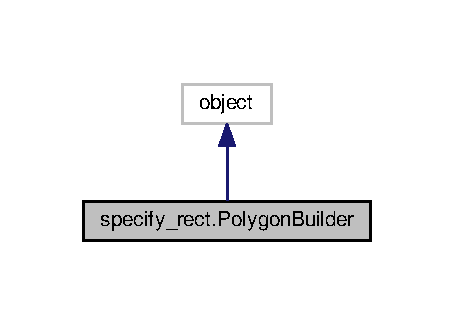
\includegraphics[width=218pt]{classspecify__rect_1_1_polygon_builder__inherit__graph}
\end{center}
\end{figure}


Collaboration diagram for specify\+\_\+rect.\+Polygon\+Builder\+:\nopagebreak
\begin{figure}[H]
\begin{center}
\leavevmode
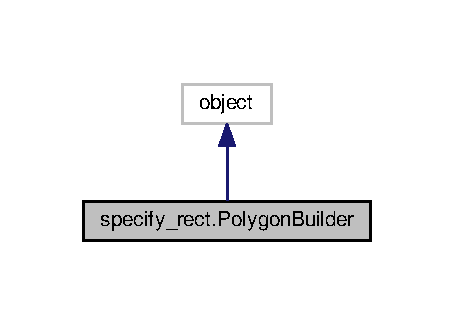
\includegraphics[width=218pt]{classspecify__rect_1_1_polygon_builder__coll__graph}
\end{center}
\end{figure}
\subsection*{Public Member Functions}
\begin{DoxyCompactItemize}
\item 
def \hyperlink{classspecify__rect_1_1_polygon_builder_aaa9568fcee5300e9b5a2cdadde5eddc4}{\+\_\+\+\_\+init\+\_\+\+\_\+} (self)
\begin{DoxyCompactList}\small\item\em Constructor. \end{DoxyCompactList}\item 
def \hyperlink{classspecify__rect_1_1_polygon_builder_a599e6951c9903fcc04da12f40451ac74}{\+\_\+\+\_\+call\+\_\+\+\_\+} (self, event)
\begin{DoxyCompactList}\small\item\em Callback function for button\+\_\+press\+\_\+event. \end{DoxyCompactList}\item 
def \hyperlink{classspecify__rect_1_1_polygon_builder_a49cc71d22b56e37306ff049108811f70}{update\+\_\+params} (self)
\begin{DoxyCompactList}\small\item\em Update values of coverage parameters. \end{DoxyCompactList}\item 
def \hyperlink{classspecify__rect_1_1_polygon_builder_a5d01b120abbd492ab7ab859b23953f73}{update\+\_\+param\+\_\+texts} (self)
\begin{DoxyCompactList}\small\item\em Update texts of coverage parameters. \end{DoxyCompactList}\item 
def \hyperlink{classspecify__rect_1_1_polygon_builder_a3a609f5f4f9a09d5fabc4b44fcaf986d}{draw\+\_\+polygon} (self, event)
\begin{DoxyCompactList}\small\item\em Callback function for \char`\"{}\+Draw Polygon\char`\"{} button. \end{DoxyCompactList}\item 
def \hyperlink{classspecify__rect_1_1_polygon_builder_aad6032c57e31102d9b5f522f3a5a88e7}{calculate\+\_\+path} (self, event)
\begin{DoxyCompactList}\small\item\em Callback function for \char`\"{}\+Calculate C\+P\char`\"{} button. \end{DoxyCompactList}\item 
def \hyperlink{classspecify__rect_1_1_polygon_builder_ae75d876010e03340950701b8f0470785}{clear\+\_\+figure} (self, event)
\begin{DoxyCompactList}\small\item\em Callback function for \char`\"{}\+Clear\char`\"{} button. \end{DoxyCompactList}\item 
def \hyperlink{classspecify__rect_1_1_polygon_builder_a712cdae443cb4478e34ffbb9aa1cbbbf}{image\+\_\+resolution\+\_\+h\+\_\+update} (self, event)
\begin{DoxyCompactList}\small\item\em Called when content of \char`\"{}\+Image Height\char`\"{} is submitted. \end{DoxyCompactList}\item 
def \hyperlink{classspecify__rect_1_1_polygon_builder_aa22d57e2c2f30a59eda71d107fc5f613}{image\+\_\+resolution\+\_\+w\+\_\+update} (self, event)
\begin{DoxyCompactList}\small\item\em Called when content of \char`\"{}\+Image Width\char`\"{} is submitted. \end{DoxyCompactList}\item 
def \hyperlink{classspecify__rect_1_1_polygon_builder_a3cd260cb4d5d11d5ae4c07140af2c8ff}{angle\+\_\+of\+\_\+view\+\_\+update} (self, event)
\begin{DoxyCompactList}\small\item\em Called when content of \char`\"{}\+Angle of view\char`\"{} is submitted. \end{DoxyCompactList}\item 
def \hyperlink{classspecify__rect_1_1_polygon_builder_a580cfa2cd0fe88cff4e3d9886256e19a}{height\+\_\+update} (self, event)
\begin{DoxyCompactList}\small\item\em Called when content of \char`\"{}\+Height\char`\"{} is submitted. \end{DoxyCompactList}\item 
def \hyperlink{classspecify__rect_1_1_polygon_builder_a22bef8c6f50d1195dc8713d2de529a8d}{horizontal\+\_\+overwrap\+\_\+update} (self, event)
\begin{DoxyCompactList}\small\item\em Called when content of \char`\"{}\+Horizontal overwrap\char`\"{} is submitted. \end{DoxyCompactList}\item 
def \hyperlink{classspecify__rect_1_1_polygon_builder_a50239e6d4954cc0d5b61404ee740a599}{vertical\+\_\+overwrap\+\_\+update} (self, event)
\begin{DoxyCompactList}\small\item\em Called when content of \char`\"{}\+Vertical overwrap\char`\"{} is submitted. \end{DoxyCompactList}\end{DoxyCompactItemize}
\subsection*{Public Attributes}
\begin{DoxyCompactItemize}
\item 
\hyperlink{classspecify__rect_1_1_polygon_builder_a5d63c74cd194ac983e9850c78cb7b3a9}{fig}
\item 
\hyperlink{classspecify__rect_1_1_polygon_builder_a2e0bae7011df2f887456db5d5929184a}{axis}
\item 
\hyperlink{classspecify__rect_1_1_polygon_builder_adfc46d632c7bd9dac9bb240a95b6c64f}{is\+\_\+polygon\+\_\+drawn}
\item 
\hyperlink{classspecify__rect_1_1_polygon_builder_a29db398c9c15e5b685ebb76543e80cd1}{server\+\_\+node}
\item 
\hyperlink{classspecify__rect_1_1_polygon_builder_a79a02e4bf8b8ff8c55150b912a0ca2d8}{lines}
\item 
\hyperlink{classspecify__rect_1_1_polygon_builder_a7bc5a210c86dc22629338c45b1b03b64}{points}
\item 
\hyperlink{classspecify__rect_1_1_polygon_builder_a7d0cd051c89820a27adcc6553effd667}{subpolygons}
\item 
\hyperlink{classspecify__rect_1_1_polygon_builder_a7327ec29baa19ea1b0d347940b4e671b}{patches}
\item 
\hyperlink{classspecify__rect_1_1_polygon_builder_a64e2c740d25d38d33e1fa903e30a5d67}{shooting\+\_\+cond}
\item 
\hyperlink{classspecify__rect_1_1_polygon_builder_a714713f2a2f6a8aad8c3649f1d0280fb}{coverage\+\_\+params}
\item 
\hyperlink{classspecify__rect_1_1_polygon_builder_a87c22817d1c77064fe3c1f72a8c8273a}{buttons}
\item 
\hyperlink{classspecify__rect_1_1_polygon_builder_a9fd3c4817fb95e2bb1015749a82d4627}{text\+\_\+boxes}
\item 
\hyperlink{classspecify__rect_1_1_polygon_builder_a4994ebc00aeb79ac5eea5b6c38785eae}{labels}
\end{DoxyCompactItemize}


\subsection{Detailed Description}
G\+UI class to specify a polygon. 

\subsection{Constructor \& Destructor Documentation}
\index{specify\+\_\+rect\+::\+Polygon\+Builder@{specify\+\_\+rect\+::\+Polygon\+Builder}!\+\_\+\+\_\+init\+\_\+\+\_\+@{\+\_\+\+\_\+init\+\_\+\+\_\+}}
\index{\+\_\+\+\_\+init\+\_\+\+\_\+@{\+\_\+\+\_\+init\+\_\+\+\_\+}!specify\+\_\+rect\+::\+Polygon\+Builder@{specify\+\_\+rect\+::\+Polygon\+Builder}}
\subsubsection[{\texorpdfstring{\+\_\+\+\_\+init\+\_\+\+\_\+(self)}{__init__(self)}}]{\setlength{\rightskip}{0pt plus 5cm}def specify\+\_\+rect.\+Polygon\+Builder.\+\_\+\+\_\+init\+\_\+\+\_\+ (
\begin{DoxyParamCaption}
\item[{}]{self}
\end{DoxyParamCaption}
)}\hypertarget{classspecify__rect_1_1_polygon_builder_aaa9568fcee5300e9b5a2cdadde5eddc4}{}\label{classspecify__rect_1_1_polygon_builder_aaa9568fcee5300e9b5a2cdadde5eddc4}


Constructor. 



\subsection{Member Function Documentation}
\index{specify\+\_\+rect\+::\+Polygon\+Builder@{specify\+\_\+rect\+::\+Polygon\+Builder}!\+\_\+\+\_\+call\+\_\+\+\_\+@{\+\_\+\+\_\+call\+\_\+\+\_\+}}
\index{\+\_\+\+\_\+call\+\_\+\+\_\+@{\+\_\+\+\_\+call\+\_\+\+\_\+}!specify\+\_\+rect\+::\+Polygon\+Builder@{specify\+\_\+rect\+::\+Polygon\+Builder}}
\subsubsection[{\texorpdfstring{\+\_\+\+\_\+call\+\_\+\+\_\+(self, event)}{__call__(self, event)}}]{\setlength{\rightskip}{0pt plus 5cm}def specify\+\_\+rect.\+Polygon\+Builder.\+\_\+\+\_\+call\+\_\+\+\_\+ (
\begin{DoxyParamCaption}
\item[{}]{self, }
\item[{}]{event}
\end{DoxyParamCaption}
)}\hypertarget{classspecify__rect_1_1_polygon_builder_a599e6951c9903fcc04da12f40451ac74}{}\label{classspecify__rect_1_1_polygon_builder_a599e6951c9903fcc04da12f40451ac74}


Callback function for button\+\_\+press\+\_\+event. 


\begin{DoxyParams}{Parameters}
{\em event} & Mouse\+Event object \\
\hline
\end{DoxyParams}
\index{specify\+\_\+rect\+::\+Polygon\+Builder@{specify\+\_\+rect\+::\+Polygon\+Builder}!angle\+\_\+of\+\_\+view\+\_\+update@{angle\+\_\+of\+\_\+view\+\_\+update}}
\index{angle\+\_\+of\+\_\+view\+\_\+update@{angle\+\_\+of\+\_\+view\+\_\+update}!specify\+\_\+rect\+::\+Polygon\+Builder@{specify\+\_\+rect\+::\+Polygon\+Builder}}
\subsubsection[{\texorpdfstring{angle\+\_\+of\+\_\+view\+\_\+update(self, event)}{angle_of_view_update(self, event)}}]{\setlength{\rightskip}{0pt plus 5cm}def specify\+\_\+rect.\+Polygon\+Builder.\+angle\+\_\+of\+\_\+view\+\_\+update (
\begin{DoxyParamCaption}
\item[{}]{self, }
\item[{}]{event}
\end{DoxyParamCaption}
)}\hypertarget{classspecify__rect_1_1_polygon_builder_a3cd260cb4d5d11d5ae4c07140af2c8ff}{}\label{classspecify__rect_1_1_polygon_builder_a3cd260cb4d5d11d5ae4c07140af2c8ff}


Called when content of \char`\"{}\+Angle of view\char`\"{} is submitted. 


\begin{DoxyParams}{Parameters}
{\em event} & Content of Text\+Box \\
\hline
\end{DoxyParams}
\index{specify\+\_\+rect\+::\+Polygon\+Builder@{specify\+\_\+rect\+::\+Polygon\+Builder}!calculate\+\_\+path@{calculate\+\_\+path}}
\index{calculate\+\_\+path@{calculate\+\_\+path}!specify\+\_\+rect\+::\+Polygon\+Builder@{specify\+\_\+rect\+::\+Polygon\+Builder}}
\subsubsection[{\texorpdfstring{calculate\+\_\+path(self, event)}{calculate_path(self, event)}}]{\setlength{\rightskip}{0pt plus 5cm}def specify\+\_\+rect.\+Polygon\+Builder.\+calculate\+\_\+path (
\begin{DoxyParamCaption}
\item[{}]{self, }
\item[{}]{event}
\end{DoxyParamCaption}
)}\hypertarget{classspecify__rect_1_1_polygon_builder_aad6032c57e31102d9b5f522f3a5a88e7}{}\label{classspecify__rect_1_1_polygon_builder_aad6032c57e31102d9b5f522f3a5a88e7}


Callback function for \char`\"{}\+Calculate C\+P\char`\"{} button. 


\begin{DoxyParams}{Parameters}
{\em event} & Mouse\+Event object \\
\hline
\end{DoxyParams}
\index{specify\+\_\+rect\+::\+Polygon\+Builder@{specify\+\_\+rect\+::\+Polygon\+Builder}!clear\+\_\+figure@{clear\+\_\+figure}}
\index{clear\+\_\+figure@{clear\+\_\+figure}!specify\+\_\+rect\+::\+Polygon\+Builder@{specify\+\_\+rect\+::\+Polygon\+Builder}}
\subsubsection[{\texorpdfstring{clear\+\_\+figure(self, event)}{clear_figure(self, event)}}]{\setlength{\rightskip}{0pt plus 5cm}def specify\+\_\+rect.\+Polygon\+Builder.\+clear\+\_\+figure (
\begin{DoxyParamCaption}
\item[{}]{self, }
\item[{}]{event}
\end{DoxyParamCaption}
)}\hypertarget{classspecify__rect_1_1_polygon_builder_ae75d876010e03340950701b8f0470785}{}\label{classspecify__rect_1_1_polygon_builder_ae75d876010e03340950701b8f0470785}


Callback function for \char`\"{}\+Clear\char`\"{} button. 


\begin{DoxyParams}{Parameters}
{\em event} & Mouse\+Event object \\
\hline
\end{DoxyParams}
\index{specify\+\_\+rect\+::\+Polygon\+Builder@{specify\+\_\+rect\+::\+Polygon\+Builder}!draw\+\_\+polygon@{draw\+\_\+polygon}}
\index{draw\+\_\+polygon@{draw\+\_\+polygon}!specify\+\_\+rect\+::\+Polygon\+Builder@{specify\+\_\+rect\+::\+Polygon\+Builder}}
\subsubsection[{\texorpdfstring{draw\+\_\+polygon(self, event)}{draw_polygon(self, event)}}]{\setlength{\rightskip}{0pt plus 5cm}def specify\+\_\+rect.\+Polygon\+Builder.\+draw\+\_\+polygon (
\begin{DoxyParamCaption}
\item[{}]{self, }
\item[{}]{event}
\end{DoxyParamCaption}
)}\hypertarget{classspecify__rect_1_1_polygon_builder_a3a609f5f4f9a09d5fabc4b44fcaf986d}{}\label{classspecify__rect_1_1_polygon_builder_a3a609f5f4f9a09d5fabc4b44fcaf986d}


Callback function for \char`\"{}\+Draw Polygon\char`\"{} button. 


\begin{DoxyParams}{Parameters}
{\em event} & Mouse\+Event object \\
\hline
\end{DoxyParams}
\index{specify\+\_\+rect\+::\+Polygon\+Builder@{specify\+\_\+rect\+::\+Polygon\+Builder}!height\+\_\+update@{height\+\_\+update}}
\index{height\+\_\+update@{height\+\_\+update}!specify\+\_\+rect\+::\+Polygon\+Builder@{specify\+\_\+rect\+::\+Polygon\+Builder}}
\subsubsection[{\texorpdfstring{height\+\_\+update(self, event)}{height_update(self, event)}}]{\setlength{\rightskip}{0pt plus 5cm}def specify\+\_\+rect.\+Polygon\+Builder.\+height\+\_\+update (
\begin{DoxyParamCaption}
\item[{}]{self, }
\item[{}]{event}
\end{DoxyParamCaption}
)}\hypertarget{classspecify__rect_1_1_polygon_builder_a580cfa2cd0fe88cff4e3d9886256e19a}{}\label{classspecify__rect_1_1_polygon_builder_a580cfa2cd0fe88cff4e3d9886256e19a}


Called when content of \char`\"{}\+Height\char`\"{} is submitted. 


\begin{DoxyParams}{Parameters}
{\em event} & Content of Text\+Box \\
\hline
\end{DoxyParams}
\index{specify\+\_\+rect\+::\+Polygon\+Builder@{specify\+\_\+rect\+::\+Polygon\+Builder}!horizontal\+\_\+overwrap\+\_\+update@{horizontal\+\_\+overwrap\+\_\+update}}
\index{horizontal\+\_\+overwrap\+\_\+update@{horizontal\+\_\+overwrap\+\_\+update}!specify\+\_\+rect\+::\+Polygon\+Builder@{specify\+\_\+rect\+::\+Polygon\+Builder}}
\subsubsection[{\texorpdfstring{horizontal\+\_\+overwrap\+\_\+update(self, event)}{horizontal_overwrap_update(self, event)}}]{\setlength{\rightskip}{0pt plus 5cm}def specify\+\_\+rect.\+Polygon\+Builder.\+horizontal\+\_\+overwrap\+\_\+update (
\begin{DoxyParamCaption}
\item[{}]{self, }
\item[{}]{event}
\end{DoxyParamCaption}
)}\hypertarget{classspecify__rect_1_1_polygon_builder_a22bef8c6f50d1195dc8713d2de529a8d}{}\label{classspecify__rect_1_1_polygon_builder_a22bef8c6f50d1195dc8713d2de529a8d}


Called when content of \char`\"{}\+Horizontal overwrap\char`\"{} is submitted. 


\begin{DoxyParams}{Parameters}
{\em event} & Content of Text\+Box \\
\hline
\end{DoxyParams}
\index{specify\+\_\+rect\+::\+Polygon\+Builder@{specify\+\_\+rect\+::\+Polygon\+Builder}!image\+\_\+resolution\+\_\+h\+\_\+update@{image\+\_\+resolution\+\_\+h\+\_\+update}}
\index{image\+\_\+resolution\+\_\+h\+\_\+update@{image\+\_\+resolution\+\_\+h\+\_\+update}!specify\+\_\+rect\+::\+Polygon\+Builder@{specify\+\_\+rect\+::\+Polygon\+Builder}}
\subsubsection[{\texorpdfstring{image\+\_\+resolution\+\_\+h\+\_\+update(self, event)}{image_resolution_h_update(self, event)}}]{\setlength{\rightskip}{0pt plus 5cm}def specify\+\_\+rect.\+Polygon\+Builder.\+image\+\_\+resolution\+\_\+h\+\_\+update (
\begin{DoxyParamCaption}
\item[{}]{self, }
\item[{}]{event}
\end{DoxyParamCaption}
)}\hypertarget{classspecify__rect_1_1_polygon_builder_a712cdae443cb4478e34ffbb9aa1cbbbf}{}\label{classspecify__rect_1_1_polygon_builder_a712cdae443cb4478e34ffbb9aa1cbbbf}


Called when content of \char`\"{}\+Image Height\char`\"{} is submitted. 


\begin{DoxyParams}{Parameters}
{\em event} & Content of Text\+Box \\
\hline
\end{DoxyParams}
\index{specify\+\_\+rect\+::\+Polygon\+Builder@{specify\+\_\+rect\+::\+Polygon\+Builder}!image\+\_\+resolution\+\_\+w\+\_\+update@{image\+\_\+resolution\+\_\+w\+\_\+update}}
\index{image\+\_\+resolution\+\_\+w\+\_\+update@{image\+\_\+resolution\+\_\+w\+\_\+update}!specify\+\_\+rect\+::\+Polygon\+Builder@{specify\+\_\+rect\+::\+Polygon\+Builder}}
\subsubsection[{\texorpdfstring{image\+\_\+resolution\+\_\+w\+\_\+update(self, event)}{image_resolution_w_update(self, event)}}]{\setlength{\rightskip}{0pt plus 5cm}def specify\+\_\+rect.\+Polygon\+Builder.\+image\+\_\+resolution\+\_\+w\+\_\+update (
\begin{DoxyParamCaption}
\item[{}]{self, }
\item[{}]{event}
\end{DoxyParamCaption}
)}\hypertarget{classspecify__rect_1_1_polygon_builder_aa22d57e2c2f30a59eda71d107fc5f613}{}\label{classspecify__rect_1_1_polygon_builder_aa22d57e2c2f30a59eda71d107fc5f613}


Called when content of \char`\"{}\+Image Width\char`\"{} is submitted. 


\begin{DoxyParams}{Parameters}
{\em event} & Content of Text\+Box \\
\hline
\end{DoxyParams}
\index{specify\+\_\+rect\+::\+Polygon\+Builder@{specify\+\_\+rect\+::\+Polygon\+Builder}!update\+\_\+param\+\_\+texts@{update\+\_\+param\+\_\+texts}}
\index{update\+\_\+param\+\_\+texts@{update\+\_\+param\+\_\+texts}!specify\+\_\+rect\+::\+Polygon\+Builder@{specify\+\_\+rect\+::\+Polygon\+Builder}}
\subsubsection[{\texorpdfstring{update\+\_\+param\+\_\+texts(self)}{update_param_texts(self)}}]{\setlength{\rightskip}{0pt plus 5cm}def specify\+\_\+rect.\+Polygon\+Builder.\+update\+\_\+param\+\_\+texts (
\begin{DoxyParamCaption}
\item[{}]{self}
\end{DoxyParamCaption}
)}\hypertarget{classspecify__rect_1_1_polygon_builder_a5d01b120abbd492ab7ab859b23953f73}{}\label{classspecify__rect_1_1_polygon_builder_a5d01b120abbd492ab7ab859b23953f73}


Update texts of coverage parameters. 

\index{specify\+\_\+rect\+::\+Polygon\+Builder@{specify\+\_\+rect\+::\+Polygon\+Builder}!update\+\_\+params@{update\+\_\+params}}
\index{update\+\_\+params@{update\+\_\+params}!specify\+\_\+rect\+::\+Polygon\+Builder@{specify\+\_\+rect\+::\+Polygon\+Builder}}
\subsubsection[{\texorpdfstring{update\+\_\+params(self)}{update_params(self)}}]{\setlength{\rightskip}{0pt plus 5cm}def specify\+\_\+rect.\+Polygon\+Builder.\+update\+\_\+params (
\begin{DoxyParamCaption}
\item[{}]{self}
\end{DoxyParamCaption}
)}\hypertarget{classspecify__rect_1_1_polygon_builder_a49cc71d22b56e37306ff049108811f70}{}\label{classspecify__rect_1_1_polygon_builder_a49cc71d22b56e37306ff049108811f70}


Update values of coverage parameters. 

\index{specify\+\_\+rect\+::\+Polygon\+Builder@{specify\+\_\+rect\+::\+Polygon\+Builder}!vertical\+\_\+overwrap\+\_\+update@{vertical\+\_\+overwrap\+\_\+update}}
\index{vertical\+\_\+overwrap\+\_\+update@{vertical\+\_\+overwrap\+\_\+update}!specify\+\_\+rect\+::\+Polygon\+Builder@{specify\+\_\+rect\+::\+Polygon\+Builder}}
\subsubsection[{\texorpdfstring{vertical\+\_\+overwrap\+\_\+update(self, event)}{vertical_overwrap_update(self, event)}}]{\setlength{\rightskip}{0pt plus 5cm}def specify\+\_\+rect.\+Polygon\+Builder.\+vertical\+\_\+overwrap\+\_\+update (
\begin{DoxyParamCaption}
\item[{}]{self, }
\item[{}]{event}
\end{DoxyParamCaption}
)}\hypertarget{classspecify__rect_1_1_polygon_builder_a50239e6d4954cc0d5b61404ee740a599}{}\label{classspecify__rect_1_1_polygon_builder_a50239e6d4954cc0d5b61404ee740a599}


Called when content of \char`\"{}\+Vertical overwrap\char`\"{} is submitted. 


\begin{DoxyParams}{Parameters}
{\em event} & Content of Text\+Box \\
\hline
\end{DoxyParams}


\subsection{Member Data Documentation}
\index{specify\+\_\+rect\+::\+Polygon\+Builder@{specify\+\_\+rect\+::\+Polygon\+Builder}!axis@{axis}}
\index{axis@{axis}!specify\+\_\+rect\+::\+Polygon\+Builder@{specify\+\_\+rect\+::\+Polygon\+Builder}}
\subsubsection[{\texorpdfstring{axis}{axis}}]{\setlength{\rightskip}{0pt plus 5cm}specify\+\_\+rect.\+Polygon\+Builder.\+axis}\hypertarget{classspecify__rect_1_1_polygon_builder_a2e0bae7011df2f887456db5d5929184a}{}\label{classspecify__rect_1_1_polygon_builder_a2e0bae7011df2f887456db5d5929184a}
\index{specify\+\_\+rect\+::\+Polygon\+Builder@{specify\+\_\+rect\+::\+Polygon\+Builder}!buttons@{buttons}}
\index{buttons@{buttons}!specify\+\_\+rect\+::\+Polygon\+Builder@{specify\+\_\+rect\+::\+Polygon\+Builder}}
\subsubsection[{\texorpdfstring{buttons}{buttons}}]{\setlength{\rightskip}{0pt plus 5cm}specify\+\_\+rect.\+Polygon\+Builder.\+buttons}\hypertarget{classspecify__rect_1_1_polygon_builder_a87c22817d1c77064fe3c1f72a8c8273a}{}\label{classspecify__rect_1_1_polygon_builder_a87c22817d1c77064fe3c1f72a8c8273a}
\index{specify\+\_\+rect\+::\+Polygon\+Builder@{specify\+\_\+rect\+::\+Polygon\+Builder}!coverage\+\_\+params@{coverage\+\_\+params}}
\index{coverage\+\_\+params@{coverage\+\_\+params}!specify\+\_\+rect\+::\+Polygon\+Builder@{specify\+\_\+rect\+::\+Polygon\+Builder}}
\subsubsection[{\texorpdfstring{coverage\+\_\+params}{coverage_params}}]{\setlength{\rightskip}{0pt plus 5cm}specify\+\_\+rect.\+Polygon\+Builder.\+coverage\+\_\+params}\hypertarget{classspecify__rect_1_1_polygon_builder_a714713f2a2f6a8aad8c3649f1d0280fb}{}\label{classspecify__rect_1_1_polygon_builder_a714713f2a2f6a8aad8c3649f1d0280fb}
\index{specify\+\_\+rect\+::\+Polygon\+Builder@{specify\+\_\+rect\+::\+Polygon\+Builder}!fig@{fig}}
\index{fig@{fig}!specify\+\_\+rect\+::\+Polygon\+Builder@{specify\+\_\+rect\+::\+Polygon\+Builder}}
\subsubsection[{\texorpdfstring{fig}{fig}}]{\setlength{\rightskip}{0pt plus 5cm}specify\+\_\+rect.\+Polygon\+Builder.\+fig}\hypertarget{classspecify__rect_1_1_polygon_builder_a5d63c74cd194ac983e9850c78cb7b3a9}{}\label{classspecify__rect_1_1_polygon_builder_a5d63c74cd194ac983e9850c78cb7b3a9}
\index{specify\+\_\+rect\+::\+Polygon\+Builder@{specify\+\_\+rect\+::\+Polygon\+Builder}!is\+\_\+polygon\+\_\+drawn@{is\+\_\+polygon\+\_\+drawn}}
\index{is\+\_\+polygon\+\_\+drawn@{is\+\_\+polygon\+\_\+drawn}!specify\+\_\+rect\+::\+Polygon\+Builder@{specify\+\_\+rect\+::\+Polygon\+Builder}}
\subsubsection[{\texorpdfstring{is\+\_\+polygon\+\_\+drawn}{is_polygon_drawn}}]{\setlength{\rightskip}{0pt plus 5cm}specify\+\_\+rect.\+Polygon\+Builder.\+is\+\_\+polygon\+\_\+drawn}\hypertarget{classspecify__rect_1_1_polygon_builder_adfc46d632c7bd9dac9bb240a95b6c64f}{}\label{classspecify__rect_1_1_polygon_builder_adfc46d632c7bd9dac9bb240a95b6c64f}
\index{specify\+\_\+rect\+::\+Polygon\+Builder@{specify\+\_\+rect\+::\+Polygon\+Builder}!labels@{labels}}
\index{labels@{labels}!specify\+\_\+rect\+::\+Polygon\+Builder@{specify\+\_\+rect\+::\+Polygon\+Builder}}
\subsubsection[{\texorpdfstring{labels}{labels}}]{\setlength{\rightskip}{0pt plus 5cm}specify\+\_\+rect.\+Polygon\+Builder.\+labels}\hypertarget{classspecify__rect_1_1_polygon_builder_a4994ebc00aeb79ac5eea5b6c38785eae}{}\label{classspecify__rect_1_1_polygon_builder_a4994ebc00aeb79ac5eea5b6c38785eae}
\index{specify\+\_\+rect\+::\+Polygon\+Builder@{specify\+\_\+rect\+::\+Polygon\+Builder}!lines@{lines}}
\index{lines@{lines}!specify\+\_\+rect\+::\+Polygon\+Builder@{specify\+\_\+rect\+::\+Polygon\+Builder}}
\subsubsection[{\texorpdfstring{lines}{lines}}]{\setlength{\rightskip}{0pt plus 5cm}specify\+\_\+rect.\+Polygon\+Builder.\+lines}\hypertarget{classspecify__rect_1_1_polygon_builder_a79a02e4bf8b8ff8c55150b912a0ca2d8}{}\label{classspecify__rect_1_1_polygon_builder_a79a02e4bf8b8ff8c55150b912a0ca2d8}
\index{specify\+\_\+rect\+::\+Polygon\+Builder@{specify\+\_\+rect\+::\+Polygon\+Builder}!patches@{patches}}
\index{patches@{patches}!specify\+\_\+rect\+::\+Polygon\+Builder@{specify\+\_\+rect\+::\+Polygon\+Builder}}
\subsubsection[{\texorpdfstring{patches}{patches}}]{\setlength{\rightskip}{0pt plus 5cm}specify\+\_\+rect.\+Polygon\+Builder.\+patches}\hypertarget{classspecify__rect_1_1_polygon_builder_a7327ec29baa19ea1b0d347940b4e671b}{}\label{classspecify__rect_1_1_polygon_builder_a7327ec29baa19ea1b0d347940b4e671b}
\index{specify\+\_\+rect\+::\+Polygon\+Builder@{specify\+\_\+rect\+::\+Polygon\+Builder}!points@{points}}
\index{points@{points}!specify\+\_\+rect\+::\+Polygon\+Builder@{specify\+\_\+rect\+::\+Polygon\+Builder}}
\subsubsection[{\texorpdfstring{points}{points}}]{\setlength{\rightskip}{0pt plus 5cm}specify\+\_\+rect.\+Polygon\+Builder.\+points}\hypertarget{classspecify__rect_1_1_polygon_builder_a7bc5a210c86dc22629338c45b1b03b64}{}\label{classspecify__rect_1_1_polygon_builder_a7bc5a210c86dc22629338c45b1b03b64}
\index{specify\+\_\+rect\+::\+Polygon\+Builder@{specify\+\_\+rect\+::\+Polygon\+Builder}!server\+\_\+node@{server\+\_\+node}}
\index{server\+\_\+node@{server\+\_\+node}!specify\+\_\+rect\+::\+Polygon\+Builder@{specify\+\_\+rect\+::\+Polygon\+Builder}}
\subsubsection[{\texorpdfstring{server\+\_\+node}{server_node}}]{\setlength{\rightskip}{0pt plus 5cm}specify\+\_\+rect.\+Polygon\+Builder.\+server\+\_\+node}\hypertarget{classspecify__rect_1_1_polygon_builder_a29db398c9c15e5b685ebb76543e80cd1}{}\label{classspecify__rect_1_1_polygon_builder_a29db398c9c15e5b685ebb76543e80cd1}
\index{specify\+\_\+rect\+::\+Polygon\+Builder@{specify\+\_\+rect\+::\+Polygon\+Builder}!shooting\+\_\+cond@{shooting\+\_\+cond}}
\index{shooting\+\_\+cond@{shooting\+\_\+cond}!specify\+\_\+rect\+::\+Polygon\+Builder@{specify\+\_\+rect\+::\+Polygon\+Builder}}
\subsubsection[{\texorpdfstring{shooting\+\_\+cond}{shooting_cond}}]{\setlength{\rightskip}{0pt plus 5cm}specify\+\_\+rect.\+Polygon\+Builder.\+shooting\+\_\+cond}\hypertarget{classspecify__rect_1_1_polygon_builder_a64e2c740d25d38d33e1fa903e30a5d67}{}\label{classspecify__rect_1_1_polygon_builder_a64e2c740d25d38d33e1fa903e30a5d67}
\index{specify\+\_\+rect\+::\+Polygon\+Builder@{specify\+\_\+rect\+::\+Polygon\+Builder}!subpolygons@{subpolygons}}
\index{subpolygons@{subpolygons}!specify\+\_\+rect\+::\+Polygon\+Builder@{specify\+\_\+rect\+::\+Polygon\+Builder}}
\subsubsection[{\texorpdfstring{subpolygons}{subpolygons}}]{\setlength{\rightskip}{0pt plus 5cm}specify\+\_\+rect.\+Polygon\+Builder.\+subpolygons}\hypertarget{classspecify__rect_1_1_polygon_builder_a7d0cd051c89820a27adcc6553effd667}{}\label{classspecify__rect_1_1_polygon_builder_a7d0cd051c89820a27adcc6553effd667}
\index{specify\+\_\+rect\+::\+Polygon\+Builder@{specify\+\_\+rect\+::\+Polygon\+Builder}!text\+\_\+boxes@{text\+\_\+boxes}}
\index{text\+\_\+boxes@{text\+\_\+boxes}!specify\+\_\+rect\+::\+Polygon\+Builder@{specify\+\_\+rect\+::\+Polygon\+Builder}}
\subsubsection[{\texorpdfstring{text\+\_\+boxes}{text_boxes}}]{\setlength{\rightskip}{0pt plus 5cm}specify\+\_\+rect.\+Polygon\+Builder.\+text\+\_\+boxes}\hypertarget{classspecify__rect_1_1_polygon_builder_a9fd3c4817fb95e2bb1015749a82d4627}{}\label{classspecify__rect_1_1_polygon_builder_a9fd3c4817fb95e2bb1015749a82d4627}


The documentation for this class was generated from the following file\+:\begin{DoxyCompactItemize}
\item 
script/\hyperlink{specify__rect_8py}{specify\+\_\+rect.\+py}\end{DoxyCompactItemize}

\chapter{File Documentation}
\hypertarget{cgutil_8hpp}{}\section{include/cgutil.hpp File Reference}
\label{cgutil_8hpp}\index{include/cgutil.\+hpp@{include/cgutil.\+hpp}}
{\ttfamily \#include $<$algorithm$>$}\\*
{\ttfamily \#include $<$cmath$>$}\\*
{\ttfamily \#include $<$list$>$}\\*
{\ttfamily \#include $<$stack$>$}\\*
{\ttfamily \#include $<$vector$>$}\\*
{\ttfamily \#include $<$C\+G\+A\+L/\+Exact\+\_\+predicates\+\_\+inexact\+\_\+constructions\+\_\+kernel.\+h$>$}\\*
{\ttfamily \#include $<$C\+G\+A\+L/\+Partition\+\_\+is\+\_\+valid\+\_\+traits\+\_\+2.\+h$>$}\\*
{\ttfamily \#include $<$C\+G\+A\+L/\+Partition\+\_\+traits\+\_\+2.\+h$>$}\\*
{\ttfamily \#include $<$C\+G\+A\+L/partition\+\_\+2.\+h$>$}\\*
{\ttfamily \#include $<$C\+G\+A\+L/point\+\_\+generators\+\_\+2.\+h$>$}\\*
{\ttfamily \#include $<$C\+G\+A\+L/polygon\+\_\+function\+\_\+objects.\+h$>$}\\*
{\ttfamily \#include $<$C\+G\+A\+L/random\+\_\+polygon\+\_\+2.\+h$>$}\\*
{\ttfamily \#include $<$ros/ros.\+h$>$}\\*
{\ttfamily \#include $<$geometry\+\_\+msgs/\+Point.\+h$>$}\\*
Include dependency graph for cgutil.\+hpp\+:\nopagebreak
\begin{figure}[H]
\begin{center}
\leavevmode
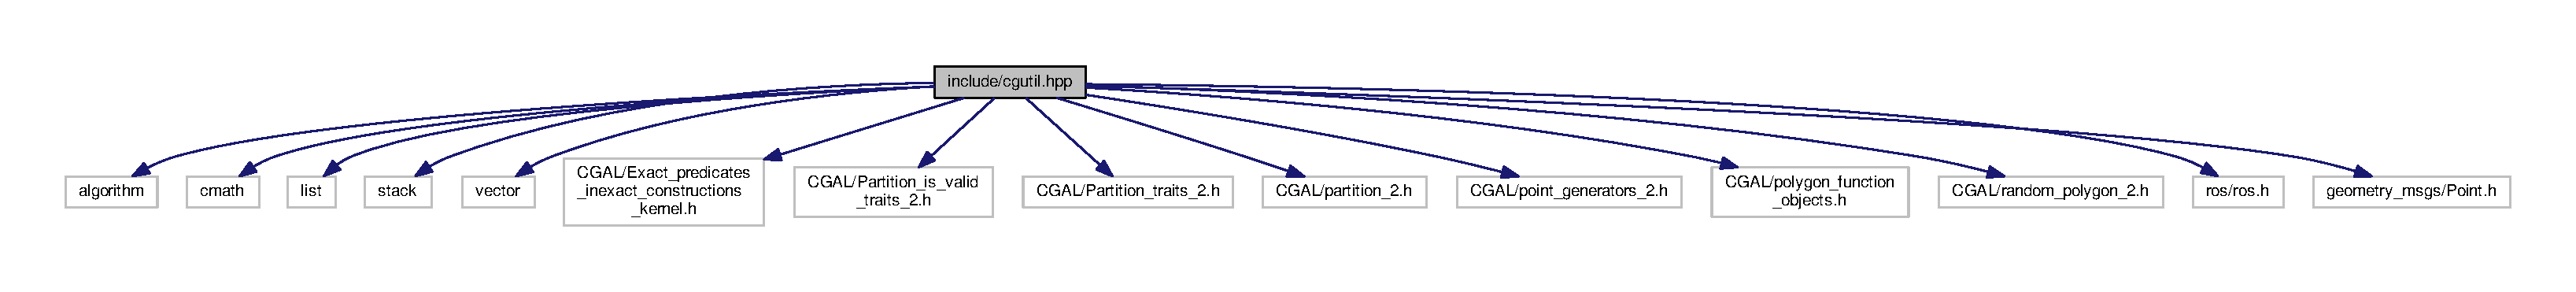
\includegraphics[width=350pt]{cgutil_8hpp__incl}
\end{center}
\end{figure}
This graph shows which files directly or indirectly include this file\+:\nopagebreak
\begin{figure}[H]
\begin{center}
\leavevmode
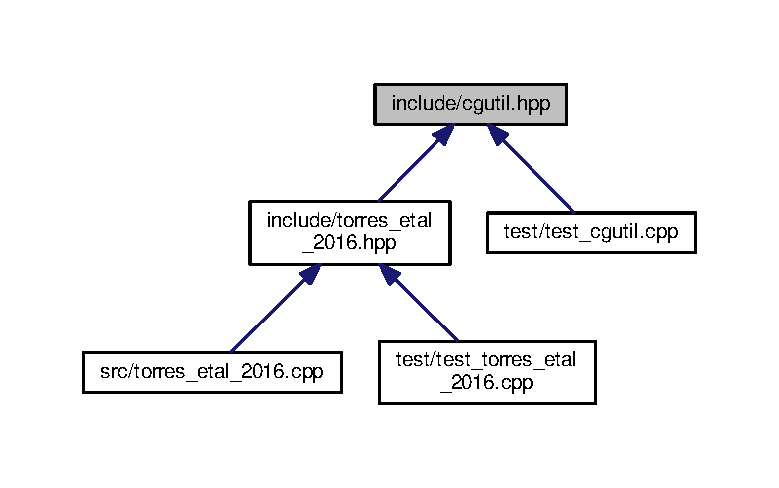
\includegraphics[width=350pt]{cgutil_8hpp__dep__incl}
\end{center}
\end{figure}
\subsection*{Typedefs}
\begin{DoxyCompactItemize}
\item 
using \hyperlink{cgutil_8hpp_a23afdbfcb523553a73b329d7a91a7489}{Point\+Vector} = std\+::vector$<$ geometry\+\_\+msgs\+::\+Point $>$
\item 
using \hyperlink{cgutil_8hpp_a7634fe1379961a22350dbd7047b2e8c1}{Line\+Segment} = std\+::array$<$ geometry\+\_\+msgs\+::\+Point, 2 $>$
\item 
using \hyperlink{cgutil_8hpp_a1b95586556e66ecbe3e4c552548d1027}{Line\+Segment\+Vector} = std\+::vector$<$ \hyperlink{cgutil_8hpp_a7634fe1379961a22350dbd7047b2e8c1}{Line\+Segment} $>$
\item 
using \hyperlink{cgutil_8hpp_ab351a84f2421d5f971fbab843bbc3a62}{K} = C\+G\+A\+L\+::\+Exact\+\_\+predicates\+\_\+inexact\+\_\+constructions\+\_\+kernel
\item 
using \hyperlink{cgutil_8hpp_a2d5e465898a6048af613458eb4b53887}{Traits} = C\+G\+A\+L\+::\+Partition\+\_\+traits\+\_\+2$<$ \hyperlink{cgutil_8hpp_ab351a84f2421d5f971fbab843bbc3a62}{K} $>$
\item 
using \hyperlink{cgutil_8hpp_a291b377e05c6893b01dfbbb4b2a383e9}{Polygon\+\_\+2} = Traits\+::\+Polygon\+\_\+2
\item 
using \hyperlink{cgutil_8hpp_a0363257d096a4b8d90de56eb63a8116e}{Point\+\_\+2} = Traits\+::\+Point\+\_\+2
\item 
using \hyperlink{cgutil_8hpp_a2f76d090b6d4623f1e9122a390d0e100}{Vertex\+\_\+iterator} = Polygon\+\_\+2\+::\+Vertex\+\_\+const\+\_\+iterator
\item 
using \hyperlink{cgutil_8hpp_a9d41026f74ac445636b2f70715c9409b}{Polygon\+\_\+list} = std\+::list$<$ \hyperlink{cgutil_8hpp_a291b377e05c6893b01dfbbb4b2a383e9}{Polygon\+\_\+2} $>$
\end{DoxyCompactItemize}
\subsection*{Functions}
\begin{DoxyCompactItemize}
\item 
double \hyperlink{cgutil_8hpp_a40332df049e2bbeebbe8c423bf33c50f}{calculate\+Signed\+Area} (const geometry\+\_\+msgs\+::\+Point \&p1, const geometry\+\_\+msgs\+::\+Point \&p2, const geometry\+\_\+msgs\+::\+Point \&p3)
\begin{DoxyCompactList}\small\item\em Calculates signed area of given triangle. \end{DoxyCompactList}\item 
bool \hyperlink{cgutil_8hpp_a518392bbc6246712757593c4ac6e6200}{operator==} (const geometry\+\_\+msgs\+::\+Point \&p1, const geometry\+\_\+msgs\+::\+Point \&p2)
\begin{DoxyCompactList}\small\item\em Check equality of two points. \end{DoxyCompactList}\item 
bool \hyperlink{cgutil_8hpp_a287adf4900c7afd5047c92bb2cd68f32}{operator!=} (const geometry\+\_\+msgs\+::\+Point \&p1, const geometry\+\_\+msgs\+::\+Point \&p2)
\begin{DoxyCompactList}\small\item\em Check equality of two points. \end{DoxyCompactList}\item 
\hyperlink{cgutil_8hpp_a1b95586556e66ecbe3e4c552548d1027}{Line\+Segment\+Vector} \hyperlink{cgutil_8hpp_acad3dc75730cb58a33626f0b922d1651}{generate\+Edge\+Vector} (const \hyperlink{cgutil_8hpp_a23afdbfcb523553a73b329d7a91a7489}{Point\+Vector} \&vec, bool is\+Closed)
\begin{DoxyCompactList}\small\item\em Generate Vector of line segment from given Point\+Vector. \end{DoxyCompactList}\item 
double \hyperlink{cgutil_8hpp_ab181ca10297ad069ba0a181734a2f4a4}{calculate\+Distance} (const geometry\+\_\+msgs\+::\+Point \&p1, const geometry\+\_\+msgs\+::\+Point \&p2)
\begin{DoxyCompactList}\small\item\em Calculates distance between given two points. \end{DoxyCompactList}\item 
double \hyperlink{cgutil_8hpp_a506da6ea8a7fafd477dd670de1d307de}{calculate\+Vertex\+Angle} (const geometry\+\_\+msgs\+::\+Point \&p1, const geometry\+\_\+msgs\+::\+Point \&p2, const geometry\+\_\+msgs\+::\+Point \&p3)
\begin{DoxyCompactList}\small\item\em Calculates angle between segment p1p2 and p1p3. \end{DoxyCompactList}\item 
double \hyperlink{cgutil_8hpp_ac682b461698a0048aa10e57b2946b34f}{calculate\+Horizontal\+Angle} (const geometry\+\_\+msgs\+::\+Point \&p1, const geometry\+\_\+msgs\+::\+Point \&p2)
\begin{DoxyCompactList}\small\item\em Calculates angle between segment p1p2 and horizontal line. \end{DoxyCompactList}\item 
double \hyperlink{cgutil_8hpp_a2603bc58792b4f2935d5462161af0cbd}{calculate\+Distance} (const \hyperlink{cgutil_8hpp_a7634fe1379961a22350dbd7047b2e8c1}{Line\+Segment} \&edge, const geometry\+\_\+msgs\+::\+Point \&vertex)
\begin{DoxyCompactList}\small\item\em Calculates distance between given edge and vertex. \end{DoxyCompactList}\item 
\hyperlink{cgutil_8hpp_a23afdbfcb523553a73b329d7a91a7489}{Point\+Vector} \hyperlink{cgutil_8hpp_a6be4127646660492844b003736100443}{compute\+Convex\+Hull} (\hyperlink{cgutil_8hpp_a23afdbfcb523553a73b329d7a91a7489}{Point\+Vector} points)
\begin{DoxyCompactList}\small\item\em Returns convex hull of given points. \end{DoxyCompactList}\item 
bool \hyperlink{cgutil_8hpp_ab3a4215076312a2435642bff1373ad40}{is\+Convex} (\hyperlink{cgutil_8hpp_a23afdbfcb523553a73b329d7a91a7489}{Point\+Vector} points)
\begin{DoxyCompactList}\small\item\em Checks if given polygon is convex or not. \end{DoxyCompactList}\item 
bool \hyperlink{cgutil_8hpp_ad3cb912330f862ac85f7ab72d121e80a}{has\+Intersection} (const \hyperlink{cgutil_8hpp_a7634fe1379961a22350dbd7047b2e8c1}{Line\+Segment} \&edge1, const \hyperlink{cgutil_8hpp_a7634fe1379961a22350dbd7047b2e8c1}{Line\+Segment} \&edge2)
\begin{DoxyCompactList}\small\item\em Checks if given edges intersect each other. \end{DoxyCompactList}\item 
bool \hyperlink{cgutil_8hpp_a75e1826df2b31502ed4961e4ec3b9058}{has\+Intersection} (const \hyperlink{cgutil_8hpp_a1b95586556e66ecbe3e4c552548d1027}{Line\+Segment\+Vector} \&vec1, const \hyperlink{cgutil_8hpp_a1b95586556e66ecbe3e4c552548d1027}{Line\+Segment\+Vector} \&vec2)
\begin{DoxyCompactList}\small\item\em Checks if given vectors of edges have at least one intersection. \end{DoxyCompactList}\item 
geometry\+\_\+msgs\+::\+Point \hyperlink{cgutil_8hpp_a1cdc17f2ebbabc6d236cfd1c45469e6e}{localize\+Intersection} (const \hyperlink{cgutil_8hpp_a7634fe1379961a22350dbd7047b2e8c1}{Line\+Segment} \&edge1, const \hyperlink{cgutil_8hpp_a7634fe1379961a22350dbd7047b2e8c1}{Line\+Segment} \&edge2)
\begin{DoxyCompactList}\small\item\em Find the location where given edges intersect each other. \end{DoxyCompactList}\item 
\hyperlink{cgutil_8hpp_a23afdbfcb523553a73b329d7a91a7489}{Point\+Vector} \hyperlink{cgutil_8hpp_af7715f8d7b828ee3f6412b2e311bd65a}{rotate\+Points} (const \hyperlink{cgutil_8hpp_a23afdbfcb523553a73b329d7a91a7489}{Point\+Vector} \&points, double angle\+\_\+rad)
\begin{DoxyCompactList}\small\item\em Rotate points by given angle around the origin. \end{DoxyCompactList}\item 
std\+::vector$<$ \hyperlink{cgutil_8hpp_a23afdbfcb523553a73b329d7a91a7489}{Point\+Vector} $>$ \hyperlink{cgutil_8hpp_a3b7a6668da8052d768b8700b096b7287}{decompose\+Polygon} (const \hyperlink{cgutil_8hpp_a23afdbfcb523553a73b329d7a91a7489}{Point\+Vector} \&polygon)
\begin{DoxyCompactList}\small\item\em Decompose given polygon. \end{DoxyCompactList}\end{DoxyCompactItemize}


\subsection{Typedef Documentation}
\index{cgutil.\+hpp@{cgutil.\+hpp}!K@{K}}
\index{K@{K}!cgutil.\+hpp@{cgutil.\+hpp}}
\subsubsection[{\texorpdfstring{K}{K}}]{\setlength{\rightskip}{0pt plus 5cm}using {\bf K} =  C\+G\+A\+L\+::\+Exact\+\_\+predicates\+\_\+inexact\+\_\+constructions\+\_\+kernel}\hypertarget{cgutil_8hpp_ab351a84f2421d5f971fbab843bbc3a62}{}\label{cgutil_8hpp_ab351a84f2421d5f971fbab843bbc3a62}
\index{cgutil.\+hpp@{cgutil.\+hpp}!Line\+Segment@{Line\+Segment}}
\index{Line\+Segment@{Line\+Segment}!cgutil.\+hpp@{cgutil.\+hpp}}
\subsubsection[{\texorpdfstring{Line\+Segment}{LineSegment}}]{\setlength{\rightskip}{0pt plus 5cm}using {\bf Line\+Segment} =  std\+::array$<$geometry\+\_\+msgs\+::\+Point, 2$>$}\hypertarget{cgutil_8hpp_a7634fe1379961a22350dbd7047b2e8c1}{}\label{cgutil_8hpp_a7634fe1379961a22350dbd7047b2e8c1}
\index{cgutil.\+hpp@{cgutil.\+hpp}!Line\+Segment\+Vector@{Line\+Segment\+Vector}}
\index{Line\+Segment\+Vector@{Line\+Segment\+Vector}!cgutil.\+hpp@{cgutil.\+hpp}}
\subsubsection[{\texorpdfstring{Line\+Segment\+Vector}{LineSegmentVector}}]{\setlength{\rightskip}{0pt plus 5cm}using {\bf Line\+Segment\+Vector} =  std\+::vector$<${\bf Line\+Segment}$>$}\hypertarget{cgutil_8hpp_a1b95586556e66ecbe3e4c552548d1027}{}\label{cgutil_8hpp_a1b95586556e66ecbe3e4c552548d1027}
\index{cgutil.\+hpp@{cgutil.\+hpp}!Point\+\_\+2@{Point\+\_\+2}}
\index{Point\+\_\+2@{Point\+\_\+2}!cgutil.\+hpp@{cgutil.\+hpp}}
\subsubsection[{\texorpdfstring{Point\+\_\+2}{Point_2}}]{\setlength{\rightskip}{0pt plus 5cm}using {\bf Point\+\_\+2} =  Traits\+::\+Point\+\_\+2}\hypertarget{cgutil_8hpp_a0363257d096a4b8d90de56eb63a8116e}{}\label{cgutil_8hpp_a0363257d096a4b8d90de56eb63a8116e}
\index{cgutil.\+hpp@{cgutil.\+hpp}!Point\+Vector@{Point\+Vector}}
\index{Point\+Vector@{Point\+Vector}!cgutil.\+hpp@{cgutil.\+hpp}}
\subsubsection[{\texorpdfstring{Point\+Vector}{PointVector}}]{\setlength{\rightskip}{0pt plus 5cm}using {\bf Point\+Vector} =  std\+::vector$<$geometry\+\_\+msgs\+::\+Point$>$}\hypertarget{cgutil_8hpp_a23afdbfcb523553a73b329d7a91a7489}{}\label{cgutil_8hpp_a23afdbfcb523553a73b329d7a91a7489}
\index{cgutil.\+hpp@{cgutil.\+hpp}!Polygon\+\_\+2@{Polygon\+\_\+2}}
\index{Polygon\+\_\+2@{Polygon\+\_\+2}!cgutil.\+hpp@{cgutil.\+hpp}}
\subsubsection[{\texorpdfstring{Polygon\+\_\+2}{Polygon_2}}]{\setlength{\rightskip}{0pt plus 5cm}using {\bf Polygon\+\_\+2} =  Traits\+::\+Polygon\+\_\+2}\hypertarget{cgutil_8hpp_a291b377e05c6893b01dfbbb4b2a383e9}{}\label{cgutil_8hpp_a291b377e05c6893b01dfbbb4b2a383e9}
\index{cgutil.\+hpp@{cgutil.\+hpp}!Polygon\+\_\+list@{Polygon\+\_\+list}}
\index{Polygon\+\_\+list@{Polygon\+\_\+list}!cgutil.\+hpp@{cgutil.\+hpp}}
\subsubsection[{\texorpdfstring{Polygon\+\_\+list}{Polygon_list}}]{\setlength{\rightskip}{0pt plus 5cm}using {\bf Polygon\+\_\+list} =  std\+::list$<${\bf Polygon\+\_\+2}$>$}\hypertarget{cgutil_8hpp_a9d41026f74ac445636b2f70715c9409b}{}\label{cgutil_8hpp_a9d41026f74ac445636b2f70715c9409b}
\index{cgutil.\+hpp@{cgutil.\+hpp}!Traits@{Traits}}
\index{Traits@{Traits}!cgutil.\+hpp@{cgutil.\+hpp}}
\subsubsection[{\texorpdfstring{Traits}{Traits}}]{\setlength{\rightskip}{0pt plus 5cm}using {\bf Traits} =  C\+G\+A\+L\+::\+Partition\+\_\+traits\+\_\+2$<${\bf K}$>$}\hypertarget{cgutil_8hpp_a2d5e465898a6048af613458eb4b53887}{}\label{cgutil_8hpp_a2d5e465898a6048af613458eb4b53887}
\index{cgutil.\+hpp@{cgutil.\+hpp}!Vertex\+\_\+iterator@{Vertex\+\_\+iterator}}
\index{Vertex\+\_\+iterator@{Vertex\+\_\+iterator}!cgutil.\+hpp@{cgutil.\+hpp}}
\subsubsection[{\texorpdfstring{Vertex\+\_\+iterator}{Vertex_iterator}}]{\setlength{\rightskip}{0pt plus 5cm}using {\bf Vertex\+\_\+iterator} =  Polygon\+\_\+2\+::\+Vertex\+\_\+const\+\_\+iterator}\hypertarget{cgutil_8hpp_a2f76d090b6d4623f1e9122a390d0e100}{}\label{cgutil_8hpp_a2f76d090b6d4623f1e9122a390d0e100}


\subsection{Function Documentation}
\index{cgutil.\+hpp@{cgutil.\+hpp}!calculate\+Distance@{calculate\+Distance}}
\index{calculate\+Distance@{calculate\+Distance}!cgutil.\+hpp@{cgutil.\+hpp}}
\subsubsection[{\texorpdfstring{calculate\+Distance(const geometry\+\_\+msgs\+::\+Point \&p1, const geometry\+\_\+msgs\+::\+Point \&p2)}{calculateDistance(const geometry_msgs::Point &p1, const geometry_msgs::Point &p2)}}]{\setlength{\rightskip}{0pt plus 5cm}double calculate\+Distance (
\begin{DoxyParamCaption}
\item[{const geometry\+\_\+msgs\+::\+Point \&}]{p1, }
\item[{const geometry\+\_\+msgs\+::\+Point \&}]{p2}
\end{DoxyParamCaption}
)\hspace{0.3cm}{\ttfamily [inline]}}\hypertarget{cgutil_8hpp_ab181ca10297ad069ba0a181734a2f4a4}{}\label{cgutil_8hpp_ab181ca10297ad069ba0a181734a2f4a4}


Calculates distance between given two points. 


\begin{DoxyParams}{Parameters}
{\em p1} & \\
\hline
{\em p2} & \\
\hline
\end{DoxyParams}
\begin{DoxyReturn}{Returns}
double Distance between two points 
\end{DoxyReturn}
\index{cgutil.\+hpp@{cgutil.\+hpp}!calculate\+Distance@{calculate\+Distance}}
\index{calculate\+Distance@{calculate\+Distance}!cgutil.\+hpp@{cgutil.\+hpp}}
\subsubsection[{\texorpdfstring{calculate\+Distance(const Line\+Segment \&edge, const geometry\+\_\+msgs\+::\+Point \&vertex)}{calculateDistance(const LineSegment &edge, const geometry_msgs::Point &vertex)}}]{\setlength{\rightskip}{0pt plus 5cm}double calculate\+Distance (
\begin{DoxyParamCaption}
\item[{const {\bf Line\+Segment} \&}]{edge, }
\item[{const geometry\+\_\+msgs\+::\+Point \&}]{vertex}
\end{DoxyParamCaption}
)}\hypertarget{cgutil_8hpp_a2603bc58792b4f2935d5462161af0cbd}{}\label{cgutil_8hpp_a2603bc58792b4f2935d5462161af0cbd}


Calculates distance between given edge and vertex. 


\begin{DoxyParams}{Parameters}
{\em edge} & An edge of given polygon \\
\hline
{\em vertex} & A vertex of given polygon \\
\hline
\end{DoxyParams}
\begin{DoxyReturn}{Returns}
double Distance between edge and vertex 
\end{DoxyReturn}
\index{cgutil.\+hpp@{cgutil.\+hpp}!calculate\+Horizontal\+Angle@{calculate\+Horizontal\+Angle}}
\index{calculate\+Horizontal\+Angle@{calculate\+Horizontal\+Angle}!cgutil.\+hpp@{cgutil.\+hpp}}
\subsubsection[{\texorpdfstring{calculate\+Horizontal\+Angle(const geometry\+\_\+msgs\+::\+Point \&p1, const geometry\+\_\+msgs\+::\+Point \&p2)}{calculateHorizontalAngle(const geometry_msgs::Point &p1, const geometry_msgs::Point &p2)}}]{\setlength{\rightskip}{0pt plus 5cm}double calculate\+Horizontal\+Angle (
\begin{DoxyParamCaption}
\item[{const geometry\+\_\+msgs\+::\+Point \&}]{p1, }
\item[{const geometry\+\_\+msgs\+::\+Point \&}]{p2}
\end{DoxyParamCaption}
)}\hypertarget{cgutil_8hpp_ac682b461698a0048aa10e57b2946b34f}{}\label{cgutil_8hpp_ac682b461698a0048aa10e57b2946b34f}


Calculates angle between segment p1p2 and horizontal line. 


\begin{DoxyParams}{Parameters}
{\em p1} & A vertex which is the origin of segment p1p2 \\
\hline
{\em p2} & The other vertex of segment p1p2 \\
\hline
\end{DoxyParams}
\begin{DoxyReturn}{Returns}
Vertex angle of p1 in radian \mbox{[}-\/pi, pi\mbox{]} 
\end{DoxyReturn}
\index{cgutil.\+hpp@{cgutil.\+hpp}!calculate\+Signed\+Area@{calculate\+Signed\+Area}}
\index{calculate\+Signed\+Area@{calculate\+Signed\+Area}!cgutil.\+hpp@{cgutil.\+hpp}}
\subsubsection[{\texorpdfstring{calculate\+Signed\+Area(const geometry\+\_\+msgs\+::\+Point \&p1, const geometry\+\_\+msgs\+::\+Point \&p2, const geometry\+\_\+msgs\+::\+Point \&p3)}{calculateSignedArea(const geometry_msgs::Point &p1, const geometry_msgs::Point &p2, const geometry_msgs::Point &p3)}}]{\setlength{\rightskip}{0pt plus 5cm}double calculate\+Signed\+Area (
\begin{DoxyParamCaption}
\item[{const geometry\+\_\+msgs\+::\+Point \&}]{p1, }
\item[{const geometry\+\_\+msgs\+::\+Point \&}]{p2, }
\item[{const geometry\+\_\+msgs\+::\+Point \&}]{p3}
\end{DoxyParamCaption}
)\hspace{0.3cm}{\ttfamily [inline]}}\hypertarget{cgutil_8hpp_a40332df049e2bbeebbe8c423bf33c50f}{}\label{cgutil_8hpp_a40332df049e2bbeebbe8c423bf33c50f}


Calculates signed area of given triangle. 


\begin{DoxyParams}{Parameters}
{\em p1} & The origin of vector $ \vec{p_1p_2} $ and $ \vec{p_1p_3} $ \\
\hline
{\em p2} & The end point of vector $ \vec{p_1p_2} $ \\
\hline
{\em p3} & The end point of vector $ \vec{p_1p_3} $ \\
\hline
\end{DoxyParams}
\begin{DoxyReturn}{Returns}
Signed area of given triangle
\end{DoxyReturn}
Signed area of triangle $ S(p1, p2, p3) $ is half of the outer product of vector $ \vec{p_1p_2} $ and $ \vec{p_1p_3} $.~\newline
 \[ S(p_1, p_2, p_3) = \frac{1}{2} \vec{p_1p_2} \times \vec{p_1p_3}\] ~\newline
And that can be written as follows,~\newline
 \begin{eqnarray*} S(p_1, p_2, p_3) & = & \frac{1}{2} \left| \begin{array}{ccc} p_1.x & p_1.y & 1 \\ p_2.x & p_2.y & 1 \\ p_3.x & p_3.y & 1 \end{array} \right| \\ & = & p_1.x(p_2.y - p_3.y) - p_1.y(p_2.x - p_3.x) - (p_2.x\times p_3.y - p_2.y\times p_3.x) \end{eqnarray*} \index{cgutil.\+hpp@{cgutil.\+hpp}!calculate\+Vertex\+Angle@{calculate\+Vertex\+Angle}}
\index{calculate\+Vertex\+Angle@{calculate\+Vertex\+Angle}!cgutil.\+hpp@{cgutil.\+hpp}}
\subsubsection[{\texorpdfstring{calculate\+Vertex\+Angle(const geometry\+\_\+msgs\+::\+Point \&p1, const geometry\+\_\+msgs\+::\+Point \&p2, const geometry\+\_\+msgs\+::\+Point \&p3)}{calculateVertexAngle(const geometry_msgs::Point &p1, const geometry_msgs::Point &p2, const geometry_msgs::Point &p3)}}]{\setlength{\rightskip}{0pt plus 5cm}double calculate\+Vertex\+Angle (
\begin{DoxyParamCaption}
\item[{const geometry\+\_\+msgs\+::\+Point \&}]{p1, }
\item[{const geometry\+\_\+msgs\+::\+Point \&}]{p2, }
\item[{const geometry\+\_\+msgs\+::\+Point \&}]{p3}
\end{DoxyParamCaption}
)}\hypertarget{cgutil_8hpp_a506da6ea8a7fafd477dd670de1d307de}{}\label{cgutil_8hpp_a506da6ea8a7fafd477dd670de1d307de}


Calculates angle between segment p1p2 and p1p3. 


\begin{DoxyParams}{Parameters}
{\em p1} & A vertex which is the origin of segment p1p2 and p1p3 \\
\hline
{\em p2} & The other point of segment p1p2 \\
\hline
{\em p3} & The other point of segment p1p3 \\
\hline
\end{DoxyParams}
\begin{DoxyReturn}{Returns}
Angle between segment p1p2 and p1p3 in radian \mbox{[}0, pi) 
\end{DoxyReturn}
\index{cgutil.\+hpp@{cgutil.\+hpp}!compute\+Convex\+Hull@{compute\+Convex\+Hull}}
\index{compute\+Convex\+Hull@{compute\+Convex\+Hull}!cgutil.\+hpp@{cgutil.\+hpp}}
\subsubsection[{\texorpdfstring{compute\+Convex\+Hull(\+Point\+Vector points)}{computeConvexHull(PointVector points)}}]{\setlength{\rightskip}{0pt plus 5cm}{\bf Point\+Vector} compute\+Convex\+Hull (
\begin{DoxyParamCaption}
\item[{{\bf Point\+Vector}}]{points}
\end{DoxyParamCaption}
)}\hypertarget{cgutil_8hpp_a6be4127646660492844b003736100443}{}\label{cgutil_8hpp_a6be4127646660492844b003736100443}


Returns convex hull of given points. 


\begin{DoxyParams}{Parameters}
{\em points} & A set of points in the plane \\
\hline
\end{DoxyParams}
\begin{DoxyReturn}{Returns}
Convex hull of given points
\end{DoxyReturn}
This function is based on graham scan algorithm \index{cgutil.\+hpp@{cgutil.\+hpp}!decompose\+Polygon@{decompose\+Polygon}}
\index{decompose\+Polygon@{decompose\+Polygon}!cgutil.\+hpp@{cgutil.\+hpp}}
\subsubsection[{\texorpdfstring{decompose\+Polygon(const Point\+Vector \&polygon)}{decomposePolygon(const PointVector &polygon)}}]{\setlength{\rightskip}{0pt plus 5cm}std\+::vector$<${\bf Point\+Vector}$>$ decompose\+Polygon (
\begin{DoxyParamCaption}
\item[{const {\bf Point\+Vector} \&}]{polygon}
\end{DoxyParamCaption}
)}\hypertarget{cgutil_8hpp_a3b7a6668da8052d768b8700b096b7287}{}\label{cgutil_8hpp_a3b7a6668da8052d768b8700b096b7287}


Decompose given polygon. 


\begin{DoxyParams}{Parameters}
{\em polygon} & Polygon to be decomposed \\
\hline
\end{DoxyParams}
\begin{DoxyReturn}{Returns}
std\+::vector$<$\+Point\+Vector$>$ Decomposed polygons  This function uses C\+G\+A\+L\+::optimal\+\_\+convex\+\_\+partition\+\_\+2 in order to perform optimal polygon decomposition. Note that this function has O(n$^\wedge$4) time complexity and O(n$^\wedge$3) space complexity. Use approx\+\_\+convex\+\_\+partition\+\_\+2 instead if the number of vertices are big because its time complexity is O(n). But apptox\+\_\+convex\+\_\+partition\+\_\+2 generates more polygons. For detail, see \href{https://doc.cgal.org/latest/Partition_2/index.html}{\tt https\+://doc.\+cgal.\+org/latest/\+Partition\+\_\+2/index.\+html} 
\end{DoxyReturn}
\index{cgutil.\+hpp@{cgutil.\+hpp}!generate\+Edge\+Vector@{generate\+Edge\+Vector}}
\index{generate\+Edge\+Vector@{generate\+Edge\+Vector}!cgutil.\+hpp@{cgutil.\+hpp}}
\subsubsection[{\texorpdfstring{generate\+Edge\+Vector(const Point\+Vector \&vec, bool is\+Closed)}{generateEdgeVector(const PointVector &vec, bool isClosed)}}]{\setlength{\rightskip}{0pt plus 5cm}{\bf Line\+Segment\+Vector} generate\+Edge\+Vector (
\begin{DoxyParamCaption}
\item[{const {\bf Point\+Vector} \&}]{vec, }
\item[{bool}]{is\+Closed}
\end{DoxyParamCaption}
)}\hypertarget{cgutil_8hpp_acad3dc75730cb58a33626f0b922d1651}{}\label{cgutil_8hpp_acad3dc75730cb58a33626f0b922d1651}


Generate Vector of line segment from given Point\+Vector. 


\begin{DoxyParams}{Parameters}
{\em vec} & \\
\hline
{\em is\+Closed} & Set true if the first point and the last are connected \\
\hline
\end{DoxyParams}
\begin{DoxyReturn}{Returns}
Line\+Segment\+Vector Vector of line segment a.\+k.\+a. std\+::vector$<$std\+::array$<$geometry\+\_\+msgs\+::\+Point, 2$>$$>$ 
\end{DoxyReturn}
\index{cgutil.\+hpp@{cgutil.\+hpp}!has\+Intersection@{has\+Intersection}}
\index{has\+Intersection@{has\+Intersection}!cgutil.\+hpp@{cgutil.\+hpp}}
\subsubsection[{\texorpdfstring{has\+Intersection(const Line\+Segment \&edge1, const Line\+Segment \&edge2)}{hasIntersection(const LineSegment &edge1, const LineSegment &edge2)}}]{\setlength{\rightskip}{0pt plus 5cm}bool has\+Intersection (
\begin{DoxyParamCaption}
\item[{const {\bf Line\+Segment} \&}]{edge1, }
\item[{const {\bf Line\+Segment} \&}]{edge2}
\end{DoxyParamCaption}
)}\hypertarget{cgutil_8hpp_ad3cb912330f862ac85f7ab72d121e80a}{}\label{cgutil_8hpp_ad3cb912330f862ac85f7ab72d121e80a}


Checks if given edges intersect each other. 


\begin{DoxyParams}{Parameters}
{\em edge1} & An edge \\
\hline
{\em edge2} & An edge \\
\hline
\end{DoxyParams}
\begin{DoxyReturn}{Returns}
True if two edges intersect 
\end{DoxyReturn}
\index{cgutil.\+hpp@{cgutil.\+hpp}!has\+Intersection@{has\+Intersection}}
\index{has\+Intersection@{has\+Intersection}!cgutil.\+hpp@{cgutil.\+hpp}}
\subsubsection[{\texorpdfstring{has\+Intersection(const Line\+Segment\+Vector \&vec1, const Line\+Segment\+Vector \&vec2)}{hasIntersection(const LineSegmentVector &vec1, const LineSegmentVector &vec2)}}]{\setlength{\rightskip}{0pt plus 5cm}bool has\+Intersection (
\begin{DoxyParamCaption}
\item[{const {\bf Line\+Segment\+Vector} \&}]{vec1, }
\item[{const {\bf Line\+Segment\+Vector} \&}]{vec2}
\end{DoxyParamCaption}
)}\hypertarget{cgutil_8hpp_a75e1826df2b31502ed4961e4ec3b9058}{}\label{cgutil_8hpp_a75e1826df2b31502ed4961e4ec3b9058}


Checks if given vectors of edges have at least one intersection. 


\begin{DoxyParams}{Parameters}
{\em vec1} & Vector of line segments \\
\hline
{\em vec2} & Vector of line segments \\
\hline
\end{DoxyParams}
\begin{DoxyReturn}{Returns}
True if given two vectors of edges have at least one intersection 
\end{DoxyReturn}
\index{cgutil.\+hpp@{cgutil.\+hpp}!is\+Convex@{is\+Convex}}
\index{is\+Convex@{is\+Convex}!cgutil.\+hpp@{cgutil.\+hpp}}
\subsubsection[{\texorpdfstring{is\+Convex(\+Point\+Vector points)}{isConvex(PointVector points)}}]{\setlength{\rightskip}{0pt plus 5cm}bool is\+Convex (
\begin{DoxyParamCaption}
\item[{{\bf Point\+Vector}}]{points}
\end{DoxyParamCaption}
)\hspace{0.3cm}{\ttfamily [inline]}}\hypertarget{cgutil_8hpp_ab3a4215076312a2435642bff1373ad40}{}\label{cgutil_8hpp_ab3a4215076312a2435642bff1373ad40}


Checks if given polygon is convex or not. 


\begin{DoxyParams}{Parameters}
{\em points} & Points consisting of polygon is to be checked \\
\hline
\end{DoxyParams}
\begin{DoxyReturn}{Returns}
True if given polygon is convex, false if it\textquotesingle{}s not convex 
\end{DoxyReturn}
\index{cgutil.\+hpp@{cgutil.\+hpp}!localize\+Intersection@{localize\+Intersection}}
\index{localize\+Intersection@{localize\+Intersection}!cgutil.\+hpp@{cgutil.\+hpp}}
\subsubsection[{\texorpdfstring{localize\+Intersection(const Line\+Segment \&edge1, const Line\+Segment \&edge2)}{localizeIntersection(const LineSegment &edge1, const LineSegment &edge2)}}]{\setlength{\rightskip}{0pt plus 5cm}geometry\+\_\+msgs\+::\+Point localize\+Intersection (
\begin{DoxyParamCaption}
\item[{const {\bf Line\+Segment} \&}]{edge1, }
\item[{const {\bf Line\+Segment} \&}]{edge2}
\end{DoxyParamCaption}
)}\hypertarget{cgutil_8hpp_a1cdc17f2ebbabc6d236cfd1c45469e6e}{}\label{cgutil_8hpp_a1cdc17f2ebbabc6d236cfd1c45469e6e}


Find the location where given edges intersect each other. 


\begin{DoxyParams}{Parameters}
{\em edge1} & \\
\hline
{\em edge2} & \\
\hline
\end{DoxyParams}
\begin{DoxyReturn}{Returns}
geometry\+\_\+msgs\+::\+Point Point of intersection  See \href{http://mf-atelier.sakura.ne.jp/mf-atelier/modules/tips/program/algorithm/a1.html}{\tt http\+://mf-\/atelier.\+sakura.\+ne.\+jp/mf-\/atelier/modules/tips/program/algorithm/a1.\+html} 
\end{DoxyReturn}
\index{cgutil.\+hpp@{cgutil.\+hpp}!operator"!=@{operator"!=}}
\index{operator"!=@{operator"!=}!cgutil.\+hpp@{cgutil.\+hpp}}
\subsubsection[{\texorpdfstring{operator"!=(const geometry\+\_\+msgs\+::\+Point \&p1, const geometry\+\_\+msgs\+::\+Point \&p2)}{operator!=(const geometry_msgs::Point &p1, const geometry_msgs::Point &p2)}}]{\setlength{\rightskip}{0pt plus 5cm}bool operator!= (
\begin{DoxyParamCaption}
\item[{const geometry\+\_\+msgs\+::\+Point \&}]{p1, }
\item[{const geometry\+\_\+msgs\+::\+Point \&}]{p2}
\end{DoxyParamCaption}
)}\hypertarget{cgutil_8hpp_a287adf4900c7afd5047c92bb2cd68f32}{}\label{cgutil_8hpp_a287adf4900c7afd5047c92bb2cd68f32}


Check equality of two points. 


\begin{DoxyParams}{Parameters}
{\em p1} & \\
\hline
{\em p2} & \\
\hline
\end{DoxyParams}
\begin{DoxyReturn}{Returns}
bool 
\end{DoxyReturn}
\index{cgutil.\+hpp@{cgutil.\+hpp}!operator==@{operator==}}
\index{operator==@{operator==}!cgutil.\+hpp@{cgutil.\+hpp}}
\subsubsection[{\texorpdfstring{operator==(const geometry\+\_\+msgs\+::\+Point \&p1, const geometry\+\_\+msgs\+::\+Point \&p2)}{operator==(const geometry_msgs::Point &p1, const geometry_msgs::Point &p2)}}]{\setlength{\rightskip}{0pt plus 5cm}bool operator== (
\begin{DoxyParamCaption}
\item[{const geometry\+\_\+msgs\+::\+Point \&}]{p1, }
\item[{const geometry\+\_\+msgs\+::\+Point \&}]{p2}
\end{DoxyParamCaption}
)}\hypertarget{cgutil_8hpp_a518392bbc6246712757593c4ac6e6200}{}\label{cgutil_8hpp_a518392bbc6246712757593c4ac6e6200}


Check equality of two points. 


\begin{DoxyParams}{Parameters}
{\em p1} & \\
\hline
{\em p2} & \\
\hline
\end{DoxyParams}
\begin{DoxyReturn}{Returns}
bool  See \href{https://stackoverflow.com/questions/4010240/comparing-doubles}{\tt https\+://stackoverflow.\+com/questions/4010240/comparing-\/doubles} 
\end{DoxyReturn}
\index{cgutil.\+hpp@{cgutil.\+hpp}!rotate\+Points@{rotate\+Points}}
\index{rotate\+Points@{rotate\+Points}!cgutil.\+hpp@{cgutil.\+hpp}}
\subsubsection[{\texorpdfstring{rotate\+Points(const Point\+Vector \&points, double angle\+\_\+rad)}{rotatePoints(const PointVector &points, double angle_rad)}}]{\setlength{\rightskip}{0pt plus 5cm}{\bf Point\+Vector} rotate\+Points (
\begin{DoxyParamCaption}
\item[{const {\bf Point\+Vector} \&}]{points, }
\item[{double}]{angle\+\_\+rad}
\end{DoxyParamCaption}
)}\hypertarget{cgutil_8hpp_af7715f8d7b828ee3f6412b2e311bd65a}{}\label{cgutil_8hpp_af7715f8d7b828ee3f6412b2e311bd65a}


Rotate points by given angle around the origin. 


\begin{DoxyParams}{Parameters}
{\em points} & Points to be rotated \\
\hline
{\em angle\+\_\+rad} & Rotation angle in radian \\
\hline
\end{DoxyParams}
\begin{DoxyReturn}{Returns}
Point\+Vector Rotated points 
\end{DoxyReturn}

\hypertarget{torres__etal__2016_8hpp}{}\section{include/torres\+\_\+etal\+\_\+2016.hpp File Reference}
\label{torres__etal__2016_8hpp}\index{include/torres\+\_\+etal\+\_\+2016.\+hpp@{include/torres\+\_\+etal\+\_\+2016.\+hpp}}


Utility for computational geometry.  


{\ttfamily \#include $<$cgutil.\+hpp$>$}\\*
{\ttfamily \#include $<$algorithm$>$}\\*
{\ttfamily \#include $<$array$>$}\\*
{\ttfamily \#include $<$cmath$>$}\\*
{\ttfamily \#include $<$string$>$}\\*
{\ttfamily \#include $<$unordered\+\_\+map$>$}\\*
{\ttfamily \#include $<$vector$>$}\\*
{\ttfamily \#include $<$boost/range/adaptor/indexed.\+hpp$>$}\\*
{\ttfamily \#include $<$boost/range/adaptor/reversed.\+hpp$>$}\\*
{\ttfamily \#include $<$ros/ros.\+h$>$}\\*
{\ttfamily \#include $<$std\+\_\+msgs/\+Float64.\+h$>$}\\*
{\ttfamily \#include $<$geometry\+\_\+msgs/\+Point.\+h$>$}\\*
Include dependency graph for torres\+\_\+etal\+\_\+2016.\+hpp\+:\nopagebreak
\begin{figure}[H]
\begin{center}
\leavevmode
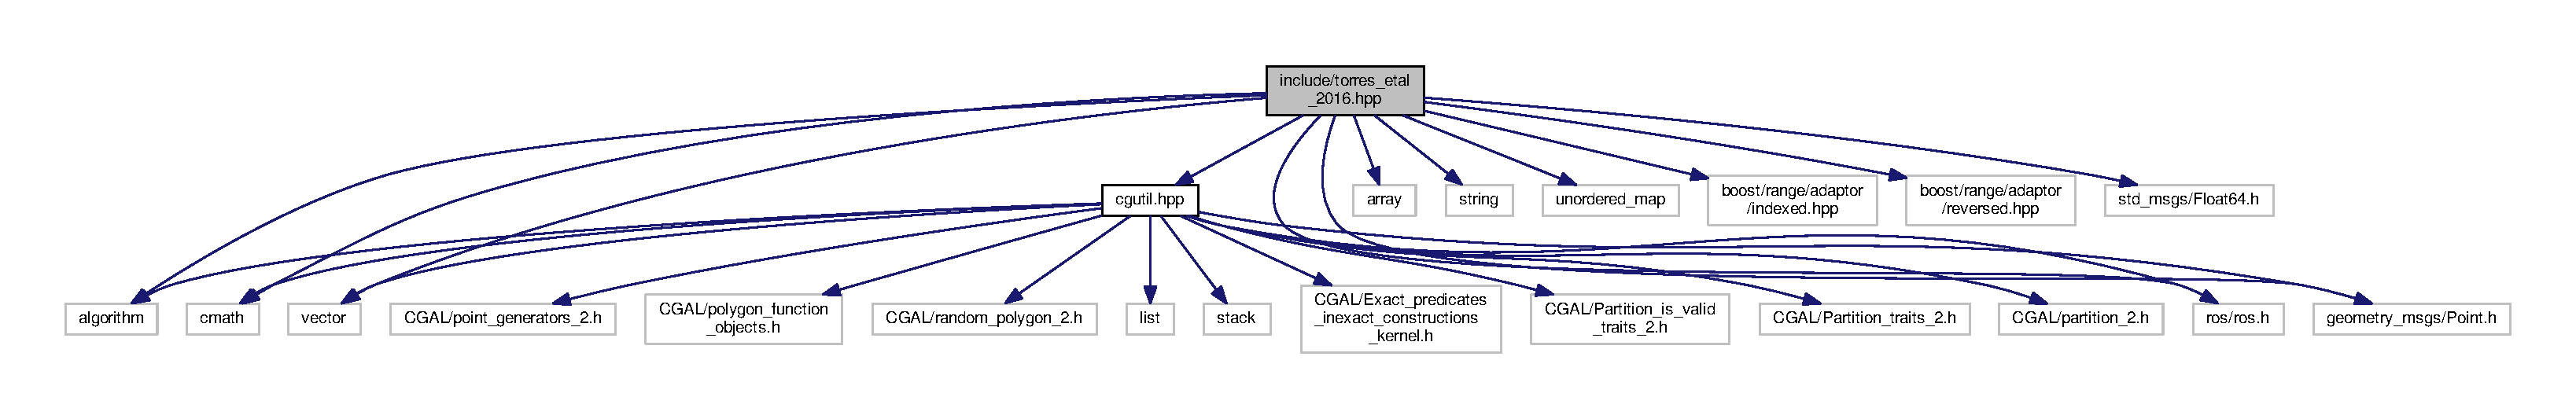
\includegraphics[width=350pt]{torres__etal__2016_8hpp__incl}
\end{center}
\end{figure}
This graph shows which files directly or indirectly include this file\+:\nopagebreak
\begin{figure}[H]
\begin{center}
\leavevmode
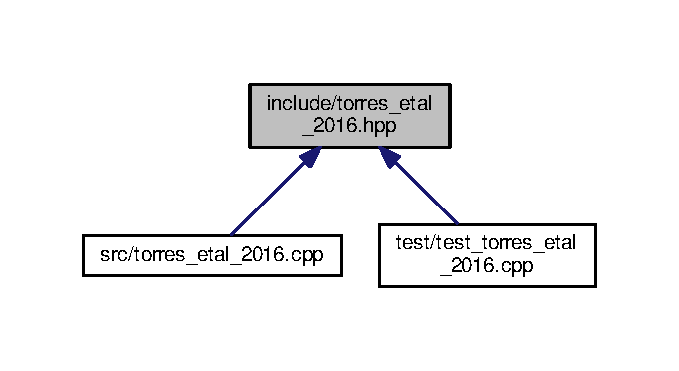
\includegraphics[width=326pt]{torres__etal__2016_8hpp__dep__incl}
\end{center}
\end{figure}
\subsection*{Classes}
\begin{DoxyCompactItemize}
\item 
struct \hyperlink{struct_direction}{Direction}
\begin{DoxyCompactList}\small\item\em Storage for line sweep direction. \end{DoxyCompactList}\end{DoxyCompactItemize}
\subsection*{Typedefs}
\begin{DoxyCompactItemize}
\item 
using \hyperlink{torres__etal__2016_8hpp_a23afdbfcb523553a73b329d7a91a7489}{Point\+Vector} = std\+::vector$<$ geometry\+\_\+msgs\+::\+Point $>$
\item 
using \hyperlink{torres__etal__2016_8hpp_a7634fe1379961a22350dbd7047b2e8c1}{Line\+Segment} = std\+::array$<$ geometry\+\_\+msgs\+::\+Point, 2 $>$
\item 
using \hyperlink{torres__etal__2016_8hpp_a1b95586556e66ecbe3e4c552548d1027}{Line\+Segment\+Vector} = std\+::vector$<$ \hyperlink{cgutil_8hpp_a7634fe1379961a22350dbd7047b2e8c1}{Line\+Segment} $>$
\end{DoxyCompactItemize}
\subsection*{Functions}
\begin{DoxyCompactItemize}
\item 
bool \hyperlink{torres__etal__2016_8hpp_adc3d848b997fd331da7d3d405b6e3c36}{is\+Clock\+Wise} (const \hyperlink{cgutil_8hpp_a23afdbfcb523553a73b329d7a91a7489}{Point\+Vector} \&path)
\begin{DoxyCompactList}\small\item\em Checks if given path is clockwise (the first turn made to the left) or not. \end{DoxyCompactList}\item 
\hyperlink{struct_direction}{Direction} \hyperlink{torres__etal__2016_8hpp_ac84e8199494b1bbdec441cf3cf5db0db}{identify\+Optimal\+Sweep\+Dir} (const \hyperlink{cgutil_8hpp_a23afdbfcb523553a73b329d7a91a7489}{Point\+Vector} \&polygon)
\begin{DoxyCompactList}\small\item\em Calculates line sweep direction for given polygon. \end{DoxyCompactList}\item 
\hyperlink{cgutil_8hpp_a23afdbfcb523553a73b329d7a91a7489}{Point\+Vector} \hyperlink{torres__etal__2016_8hpp_a0daa54859a24719e9ef5c4d957ad864f}{reshape\+Path} (const \hyperlink{cgutil_8hpp_a23afdbfcb523553a73b329d7a91a7489}{Point\+Vector} \&path, double padding)
\begin{DoxyCompactList}\small\item\em Reshape given path. \end{DoxyCompactList}\item 
bool \hyperlink{torres__etal__2016_8hpp_a340e8ecb91a252b4343c57f01ace7130}{compute\+Convex\+Coverage} (const \hyperlink{cgutil_8hpp_a23afdbfcb523553a73b329d7a91a7489}{Point\+Vector} \&polygon, double footprint\+Width, double horizontal\+Overwrap, const \hyperlink{struct_direction}{Direction} \&sweep\+Direction, \hyperlink{cgutil_8hpp_a23afdbfcb523553a73b329d7a91a7489}{Point\+Vector} \&path)
\begin{DoxyCompactList}\small\item\em Compute coverage path for convex polygon. \end{DoxyCompactList}\item 
bool \hyperlink{torres__etal__2016_8hpp_a10cafc27ed2f11edf912c94e7f30107e}{compute\+Convex\+Coverage} (const \hyperlink{cgutil_8hpp_a23afdbfcb523553a73b329d7a91a7489}{Point\+Vector} \&polygon, double footprint\+Width, double horizontal\+Overwrap, \hyperlink{cgutil_8hpp_a23afdbfcb523553a73b329d7a91a7489}{Point\+Vector} \&path)
\begin{DoxyCompactList}\small\item\em Compute coverage path for convex polygon. \end{DoxyCompactList}\item 
double \hyperlink{torres__etal__2016_8hpp_a03113b9a489d4c5846eadfa4576ce7e3}{calculate\+Path\+Length} (const \hyperlink{cgutil_8hpp_a23afdbfcb523553a73b329d7a91a7489}{Point\+Vector} \&path)
\begin{DoxyCompactList}\small\item\em Calculates length of path. \end{DoxyCompactList}\item 
\hyperlink{cgutil_8hpp_a23afdbfcb523553a73b329d7a91a7489}{Point\+Vector} \hyperlink{torres__etal__2016_8hpp_a71b7a534df669e33077111195cb5cc4b}{compute\+C\+C\+W\+Path} (\hyperlink{cgutil_8hpp_a23afdbfcb523553a73b329d7a91a7489}{Point\+Vector} path)
\begin{DoxyCompactList}\small\item\em Return counter clock wise-\/ed path of given path. \end{DoxyCompactList}\item 
\hyperlink{cgutil_8hpp_a23afdbfcb523553a73b329d7a91a7489}{Point\+Vector} \hyperlink{torres__etal__2016_8hpp_afa4eb774c5f34b95abf1e450602f9ada}{compute\+Opposite\+Path} (const \hyperlink{cgutil_8hpp_a23afdbfcb523553a73b329d7a91a7489}{Point\+Vector} \&path)
\begin{DoxyCompactList}\small\item\em Return opposite path of given path. \end{DoxyCompactList}\item 
\hyperlink{cgutil_8hpp_a23afdbfcb523553a73b329d7a91a7489}{Point\+Vector} \hyperlink{torres__etal__2016_8hpp_af347c57b74f9db063c89d01151933e29}{identify\+Optimal\+Alternative} (const \hyperlink{cgutil_8hpp_a23afdbfcb523553a73b329d7a91a7489}{Point\+Vector} \&polygon, const \hyperlink{cgutil_8hpp_a23afdbfcb523553a73b329d7a91a7489}{Point\+Vector} \&path, const geometry\+\_\+msgs\+::\+Point \&start, const geometry\+\_\+msgs\+::\+Point \&end)
\begin{DoxyCompactList}\small\item\em Identify optimal path from 4 coverage alternatives. \end{DoxyCompactList}\item 
\hyperlink{cgutil_8hpp_a23afdbfcb523553a73b329d7a91a7489}{Point\+Vector} \hyperlink{torres__etal__2016_8hpp_a012334ffd93ffb76acb1a8d31984721e}{identify\+Optimal\+Alternative} (const \hyperlink{cgutil_8hpp_a23afdbfcb523553a73b329d7a91a7489}{Point\+Vector} \&polygon, const \hyperlink{cgutil_8hpp_a23afdbfcb523553a73b329d7a91a7489}{Point\+Vector} \&path, const geometry\+\_\+msgs\+::\+Point \&start)
\begin{DoxyCompactList}\small\item\em Identify optimal path from 4 coverage alternatives. \end{DoxyCompactList}\item 
bool \hyperlink{torres__etal__2016_8hpp_a7a55117d4e1bdfc6a402f62db41b5024}{find\+Second\+Optimal\+Path} (const \hyperlink{cgutil_8hpp_a23afdbfcb523553a73b329d7a91a7489}{Point\+Vector} \&polygon, double footprint\+Width, double horizontal\+Overwrap, \hyperlink{cgutil_8hpp_a23afdbfcb523553a73b329d7a91a7489}{Point\+Vector} \&path)
\begin{DoxyCompactList}\small\item\em Find second optimal path. \end{DoxyCompactList}\item 
bool \hyperlink{torres__etal__2016_8hpp_aee24dd72675dcde2c3ad1930e2cf4658}{is\+Adjacent} (const \hyperlink{cgutil_8hpp_a23afdbfcb523553a73b329d7a91a7489}{Point\+Vector} \&polygon1, const \hyperlink{cgutil_8hpp_a23afdbfcb523553a73b329d7a91a7489}{Point\+Vector} \&polygon2)
\begin{DoxyCompactList}\small\item\em Check if given two polygons are adjacent. \end{DoxyCompactList}\item 
\hyperlink{cgutil_8hpp_a23afdbfcb523553a73b329d7a91a7489}{Point\+Vector} \hyperlink{torres__etal__2016_8hpp_a20fa2d4d482ca06a8f9956491237699c}{compute\+Multiple\+Polygon\+Coverage} (std\+::vector$<$ \hyperlink{cgutil_8hpp_a23afdbfcb523553a73b329d7a91a7489}{Point\+Vector} $>$ sub\+Polygons, double footprint\+Width, double horizontal\+Overwrap, int adjacency\+Criteria=1)
\begin{DoxyCompactList}\small\item\em Compute coverage path for multiple convex polygons. \end{DoxyCompactList}\end{DoxyCompactItemize}


\subsection{Detailed Description}
Utility for computational geometry. 

Header file for \hyperlink{torres__etal__2016_8cpp}{torres\+\_\+etal\+\_\+2016.\+cpp}.

\begin{DoxyAuthor}{Author}
Takaki Ueno 
\end{DoxyAuthor}


\subsection{Typedef Documentation}
\index{torres\+\_\+etal\+\_\+2016.\+hpp@{torres\+\_\+etal\+\_\+2016.\+hpp}!Line\+Segment@{Line\+Segment}}
\index{Line\+Segment@{Line\+Segment}!torres\+\_\+etal\+\_\+2016.\+hpp@{torres\+\_\+etal\+\_\+2016.\+hpp}}
\subsubsection[{\texorpdfstring{Line\+Segment}{LineSegment}}]{\setlength{\rightskip}{0pt plus 5cm}using {\bf Line\+Segment} =  std\+::array$<$geometry\+\_\+msgs\+::\+Point, 2$>$}\hypertarget{torres__etal__2016_8hpp_a7634fe1379961a22350dbd7047b2e8c1}{}\label{torres__etal__2016_8hpp_a7634fe1379961a22350dbd7047b2e8c1}
\index{torres\+\_\+etal\+\_\+2016.\+hpp@{torres\+\_\+etal\+\_\+2016.\+hpp}!Line\+Segment\+Vector@{Line\+Segment\+Vector}}
\index{Line\+Segment\+Vector@{Line\+Segment\+Vector}!torres\+\_\+etal\+\_\+2016.\+hpp@{torres\+\_\+etal\+\_\+2016.\+hpp}}
\subsubsection[{\texorpdfstring{Line\+Segment\+Vector}{LineSegmentVector}}]{\setlength{\rightskip}{0pt plus 5cm}using {\bf Line\+Segment\+Vector} =  std\+::vector$<${\bf Line\+Segment}$>$}\hypertarget{torres__etal__2016_8hpp_a1b95586556e66ecbe3e4c552548d1027}{}\label{torres__etal__2016_8hpp_a1b95586556e66ecbe3e4c552548d1027}
\index{torres\+\_\+etal\+\_\+2016.\+hpp@{torres\+\_\+etal\+\_\+2016.\+hpp}!Point\+Vector@{Point\+Vector}}
\index{Point\+Vector@{Point\+Vector}!torres\+\_\+etal\+\_\+2016.\+hpp@{torres\+\_\+etal\+\_\+2016.\+hpp}}
\subsubsection[{\texorpdfstring{Point\+Vector}{PointVector}}]{\setlength{\rightskip}{0pt plus 5cm}using {\bf Point\+Vector} =  std\+::vector$<$geometry\+\_\+msgs\+::\+Point$>$}\hypertarget{torres__etal__2016_8hpp_a23afdbfcb523553a73b329d7a91a7489}{}\label{torres__etal__2016_8hpp_a23afdbfcb523553a73b329d7a91a7489}


\subsection{Function Documentation}
\index{torres\+\_\+etal\+\_\+2016.\+hpp@{torres\+\_\+etal\+\_\+2016.\+hpp}!calculate\+Path\+Length@{calculate\+Path\+Length}}
\index{calculate\+Path\+Length@{calculate\+Path\+Length}!torres\+\_\+etal\+\_\+2016.\+hpp@{torres\+\_\+etal\+\_\+2016.\+hpp}}
\subsubsection[{\texorpdfstring{calculate\+Path\+Length(const Point\+Vector \&path)}{calculatePathLength(const PointVector &path)}}]{\setlength{\rightskip}{0pt plus 5cm}double calculate\+Path\+Length (
\begin{DoxyParamCaption}
\item[{const {\bf Point\+Vector} \&}]{path}
\end{DoxyParamCaption}
)}\hypertarget{torres__etal__2016_8hpp_a03113b9a489d4c5846eadfa4576ce7e3}{}\label{torres__etal__2016_8hpp_a03113b9a489d4c5846eadfa4576ce7e3}


Calculates length of path. 


\begin{DoxyParams}{Parameters}
{\em path} & \\
\hline
\end{DoxyParams}
\begin{DoxyReturn}{Returns}
double Length of path 
\end{DoxyReturn}
\index{torres\+\_\+etal\+\_\+2016.\+hpp@{torres\+\_\+etal\+\_\+2016.\+hpp}!compute\+C\+C\+W\+Path@{compute\+C\+C\+W\+Path}}
\index{compute\+C\+C\+W\+Path@{compute\+C\+C\+W\+Path}!torres\+\_\+etal\+\_\+2016.\+hpp@{torres\+\_\+etal\+\_\+2016.\+hpp}}
\subsubsection[{\texorpdfstring{compute\+C\+C\+W\+Path(\+Point\+Vector path)}{computeCCWPath(PointVector path)}}]{\setlength{\rightskip}{0pt plus 5cm}{\bf Point\+Vector} compute\+C\+C\+W\+Path (
\begin{DoxyParamCaption}
\item[{{\bf Point\+Vector}}]{path}
\end{DoxyParamCaption}
)}\hypertarget{torres__etal__2016_8hpp_a71b7a534df669e33077111195cb5cc4b}{}\label{torres__etal__2016_8hpp_a71b7a534df669e33077111195cb5cc4b}


Return counter clock wise-\/ed path of given path. 


\begin{DoxyParams}{Parameters}
{\em path} & Clockwise path \\
\hline
\end{DoxyParams}
\begin{DoxyReturn}{Returns}
Point\+Vector Counter clock wise version of given path 
\end{DoxyReturn}
\index{torres\+\_\+etal\+\_\+2016.\+hpp@{torres\+\_\+etal\+\_\+2016.\+hpp}!compute\+Convex\+Coverage@{compute\+Convex\+Coverage}}
\index{compute\+Convex\+Coverage@{compute\+Convex\+Coverage}!torres\+\_\+etal\+\_\+2016.\+hpp@{torres\+\_\+etal\+\_\+2016.\+hpp}}
\subsubsection[{\texorpdfstring{compute\+Convex\+Coverage(const Point\+Vector \&polygon, double footprint\+Width, double horizontal\+Overwrap, const Direction \&sweep\+Direction, Point\+Vector \&path)}{computeConvexCoverage(const PointVector &polygon, double footprintWidth, double horizontalOverwrap, const Direction &sweepDirection, PointVector &path)}}]{\setlength{\rightskip}{0pt plus 5cm}bool compute\+Convex\+Coverage (
\begin{DoxyParamCaption}
\item[{const {\bf Point\+Vector} \&}]{polygon, }
\item[{double}]{footprint\+Width, }
\item[{double}]{horizontal\+Overwrap, }
\item[{const {\bf Direction} \&}]{sweep\+Direction, }
\item[{{\bf Point\+Vector} \&}]{path}
\end{DoxyParamCaption}
)}\hypertarget{torres__etal__2016_8hpp_a340e8ecb91a252b4343c57f01ace7130}{}\label{torres__etal__2016_8hpp_a340e8ecb91a252b4343c57f01ace7130}


Compute coverage path for convex polygon. 


\begin{DoxyParams}{Parameters}
{\em polygon} & Coverage path is calculated on this region \\
\hline
{\em footprint\+Width} & Width of the area taken by one sweep \\
\hline
{\em horizontal\+Overwrap} & Horizontal overwrap of each sweep \\
\hline
{\em sweep\+Direction} & \\
\hline
{\em path} & Path of coverage path \\
\hline
\end{DoxyParams}
\begin{DoxyReturn}{Returns}
bool True if path does not intersect with polygon 
\end{DoxyReturn}
\index{torres\+\_\+etal\+\_\+2016.\+hpp@{torres\+\_\+etal\+\_\+2016.\+hpp}!compute\+Convex\+Coverage@{compute\+Convex\+Coverage}}
\index{compute\+Convex\+Coverage@{compute\+Convex\+Coverage}!torres\+\_\+etal\+\_\+2016.\+hpp@{torres\+\_\+etal\+\_\+2016.\+hpp}}
\subsubsection[{\texorpdfstring{compute\+Convex\+Coverage(const Point\+Vector \&polygon, double footprint\+Width, double horizontal\+Overwrap, Point\+Vector \&path)}{computeConvexCoverage(const PointVector &polygon, double footprintWidth, double horizontalOverwrap, PointVector &path)}}]{\setlength{\rightskip}{0pt plus 5cm}bool compute\+Convex\+Coverage (
\begin{DoxyParamCaption}
\item[{const {\bf Point\+Vector} \&}]{polygon, }
\item[{double}]{footprint\+Width, }
\item[{double}]{horizontal\+Overwrap, }
\item[{{\bf Point\+Vector} \&}]{path}
\end{DoxyParamCaption}
)}\hypertarget{torres__etal__2016_8hpp_a10cafc27ed2f11edf912c94e7f30107e}{}\label{torres__etal__2016_8hpp_a10cafc27ed2f11edf912c94e7f30107e}


Compute coverage path for convex polygon. 


\begin{DoxyParams}{Parameters}
{\em polygon} & Coverage path is calculated on this region \\
\hline
{\em footprint\+Width} & Width of the area taken by one sweep \\
\hline
{\em horizontal\+Overwrap} & Horizontal overwrap of each sweep \\
\hline
{\em path} & Path of coverage path \\
\hline
\end{DoxyParams}
\begin{DoxyReturn}{Returns}
bool True if path does not intersect with polygon 
\end{DoxyReturn}
\index{torres\+\_\+etal\+\_\+2016.\+hpp@{torres\+\_\+etal\+\_\+2016.\+hpp}!compute\+Multiple\+Polygon\+Coverage@{compute\+Multiple\+Polygon\+Coverage}}
\index{compute\+Multiple\+Polygon\+Coverage@{compute\+Multiple\+Polygon\+Coverage}!torres\+\_\+etal\+\_\+2016.\+hpp@{torres\+\_\+etal\+\_\+2016.\+hpp}}
\subsubsection[{\texorpdfstring{compute\+Multiple\+Polygon\+Coverage(std\+::vector$<$ Point\+Vector $>$ sub\+Polygons, double footprint\+Width, double horizontal\+Overwrap, int adjacency\+Criteria=1)}{computeMultiplePolygonCoverage(std::vector< PointVector > subPolygons, double footprintWidth, double horizontalOverwrap, int adjacencyCriteria=1)}}]{\setlength{\rightskip}{0pt plus 5cm}{\bf Point\+Vector} compute\+Multiple\+Polygon\+Coverage (
\begin{DoxyParamCaption}
\item[{std\+::vector$<$ {\bf Point\+Vector} $>$}]{sub\+Polygons, }
\item[{double}]{footprint\+Width, }
\item[{double}]{horizontal\+Overwrap, }
\item[{int}]{adjacency\+Criteria = {\ttfamily 1}}
\end{DoxyParamCaption}
)}\hypertarget{torres__etal__2016_8hpp_a20fa2d4d482ca06a8f9956491237699c}{}\label{torres__etal__2016_8hpp_a20fa2d4d482ca06a8f9956491237699c}


Compute coverage path for multiple convex polygons. 


\begin{DoxyParams}{Parameters}
{\em sub\+Polygons} & \\
\hline
{\em footprint\+Width} & \\
\hline
{\em horizontal\+Overwrap} & \\
\hline
{\em adjacency\+Criteria} & Ignore paths which have less adjacent polygons than this number \\
\hline
\end{DoxyParams}
\begin{DoxyReturn}{Returns}
Point\+Vector Computed Path  See section 6.\+2 of torres et al. 2016 for the detail 
\end{DoxyReturn}
\index{torres\+\_\+etal\+\_\+2016.\+hpp@{torres\+\_\+etal\+\_\+2016.\+hpp}!compute\+Opposite\+Path@{compute\+Opposite\+Path}}
\index{compute\+Opposite\+Path@{compute\+Opposite\+Path}!torres\+\_\+etal\+\_\+2016.\+hpp@{torres\+\_\+etal\+\_\+2016.\+hpp}}
\subsubsection[{\texorpdfstring{compute\+Opposite\+Path(const Point\+Vector \&path)}{computeOppositePath(const PointVector &path)}}]{\setlength{\rightskip}{0pt plus 5cm}{\bf Point\+Vector} compute\+Opposite\+Path (
\begin{DoxyParamCaption}
\item[{const {\bf Point\+Vector} \&}]{path}
\end{DoxyParamCaption}
)}\hypertarget{torres__etal__2016_8hpp_afa4eb774c5f34b95abf1e450602f9ada}{}\label{torres__etal__2016_8hpp_afa4eb774c5f34b95abf1e450602f9ada}


Return opposite path of given path. 


\begin{DoxyParams}{Parameters}
{\em path} & \\
\hline
\end{DoxyParams}
\begin{DoxyReturn}{Returns}
Point\+Vector Path with points of reversed order of given path 
\end{DoxyReturn}
\index{torres\+\_\+etal\+\_\+2016.\+hpp@{torres\+\_\+etal\+\_\+2016.\+hpp}!find\+Second\+Optimal\+Path@{find\+Second\+Optimal\+Path}}
\index{find\+Second\+Optimal\+Path@{find\+Second\+Optimal\+Path}!torres\+\_\+etal\+\_\+2016.\+hpp@{torres\+\_\+etal\+\_\+2016.\+hpp}}
\subsubsection[{\texorpdfstring{find\+Second\+Optimal\+Path(const Point\+Vector \&polygon, double footprint\+Width, double horizontal\+Overwrap, Point\+Vector \&path)}{findSecondOptimalPath(const PointVector &polygon, double footprintWidth, double horizontalOverwrap, PointVector &path)}}]{\setlength{\rightskip}{0pt plus 5cm}bool find\+Second\+Optimal\+Path (
\begin{DoxyParamCaption}
\item[{const {\bf Point\+Vector} \&}]{polygon, }
\item[{double}]{footprint\+Width, }
\item[{double}]{horizontal\+Overwrap, }
\item[{{\bf Point\+Vector} \&}]{path}
\end{DoxyParamCaption}
)}\hypertarget{torres__etal__2016_8hpp_a7a55117d4e1bdfc6a402f62db41b5024}{}\label{torres__etal__2016_8hpp_a7a55117d4e1bdfc6a402f62db41b5024}


Find second optimal path. 


\begin{DoxyParams}{Parameters}
{\em polygon} & \\
\hline
{\em footprint\+Width} & \\
\hline
{\em horizontal\+Overwrap} & \\
\hline
{\em path} & \\
\hline
\end{DoxyParams}
\begin{DoxyReturn}{Returns}
bool True if second optimal path exists 
\end{DoxyReturn}
\index{torres\+\_\+etal\+\_\+2016.\+hpp@{torres\+\_\+etal\+\_\+2016.\+hpp}!identify\+Optimal\+Alternative@{identify\+Optimal\+Alternative}}
\index{identify\+Optimal\+Alternative@{identify\+Optimal\+Alternative}!torres\+\_\+etal\+\_\+2016.\+hpp@{torres\+\_\+etal\+\_\+2016.\+hpp}}
\subsubsection[{\texorpdfstring{identify\+Optimal\+Alternative(const Point\+Vector \&polygon, const Point\+Vector \&path, const geometry\+\_\+msgs\+::\+Point \&start, const geometry\+\_\+msgs\+::\+Point \&end)}{identifyOptimalAlternative(const PointVector &polygon, const PointVector &path, const geometry_msgs::Point &start, const geometry_msgs::Point &end)}}]{\setlength{\rightskip}{0pt plus 5cm}{\bf Point\+Vector} identify\+Optimal\+Alternative (
\begin{DoxyParamCaption}
\item[{const {\bf Point\+Vector} \&}]{polygon, }
\item[{const {\bf Point\+Vector} \&}]{path, }
\item[{const geometry\+\_\+msgs\+::\+Point \&}]{start, }
\item[{const geometry\+\_\+msgs\+::\+Point \&}]{end}
\end{DoxyParamCaption}
)}\hypertarget{torres__etal__2016_8hpp_af347c57b74f9db063c89d01151933e29}{}\label{torres__etal__2016_8hpp_af347c57b74f9db063c89d01151933e29}


Identify optimal path from 4 coverage alternatives. 


\begin{DoxyParams}{Parameters}
{\em polygon} & \\
\hline
{\em path} & \\
\hline
{\em start} & Start point \\
\hline
{\em end} & End point \\
\hline
\end{DoxyParams}
\begin{DoxyReturn}{Returns}
Point\+Vector Optimal path that minimizes the length of path  The naming of the following variable follows torres et al. 2016 
\end{DoxyReturn}
\index{torres\+\_\+etal\+\_\+2016.\+hpp@{torres\+\_\+etal\+\_\+2016.\+hpp}!identify\+Optimal\+Alternative@{identify\+Optimal\+Alternative}}
\index{identify\+Optimal\+Alternative@{identify\+Optimal\+Alternative}!torres\+\_\+etal\+\_\+2016.\+hpp@{torres\+\_\+etal\+\_\+2016.\+hpp}}
\subsubsection[{\texorpdfstring{identify\+Optimal\+Alternative(const Point\+Vector \&polygon, const Point\+Vector \&path, const geometry\+\_\+msgs\+::\+Point \&start)}{identifyOptimalAlternative(const PointVector &polygon, const PointVector &path, const geometry_msgs::Point &start)}}]{\setlength{\rightskip}{0pt plus 5cm}{\bf Point\+Vector} identify\+Optimal\+Alternative (
\begin{DoxyParamCaption}
\item[{const {\bf Point\+Vector} \&}]{polygon, }
\item[{const {\bf Point\+Vector} \&}]{path, }
\item[{const geometry\+\_\+msgs\+::\+Point \&}]{start}
\end{DoxyParamCaption}
)}\hypertarget{torres__etal__2016_8hpp_a012334ffd93ffb76acb1a8d31984721e}{}\label{torres__etal__2016_8hpp_a012334ffd93ffb76acb1a8d31984721e}


Identify optimal path from 4 coverage alternatives. 


\begin{DoxyParams}{Parameters}
{\em polygon} & \\
\hline
{\em path} & \\
\hline
{\em start} & Start point \\
\hline
\end{DoxyParams}
\begin{DoxyReturn}{Returns}
Point\+Vector Optimal path that minimizes the length of path  The naming of the following variable follows torres et al. 2016 
\end{DoxyReturn}
\index{torres\+\_\+etal\+\_\+2016.\+hpp@{torres\+\_\+etal\+\_\+2016.\+hpp}!identify\+Optimal\+Sweep\+Dir@{identify\+Optimal\+Sweep\+Dir}}
\index{identify\+Optimal\+Sweep\+Dir@{identify\+Optimal\+Sweep\+Dir}!torres\+\_\+etal\+\_\+2016.\+hpp@{torres\+\_\+etal\+\_\+2016.\+hpp}}
\subsubsection[{\texorpdfstring{identify\+Optimal\+Sweep\+Dir(const Point\+Vector \&polygon)}{identifyOptimalSweepDir(const PointVector &polygon)}}]{\setlength{\rightskip}{0pt plus 5cm}{\bf Direction} identify\+Optimal\+Sweep\+Dir (
\begin{DoxyParamCaption}
\item[{const {\bf Point\+Vector} \&}]{polygon}
\end{DoxyParamCaption}
)}\hypertarget{torres__etal__2016_8hpp_ac84e8199494b1bbdec441cf3cf5db0db}{}\label{torres__etal__2016_8hpp_ac84e8199494b1bbdec441cf3cf5db0db}


Calculates line sweep direction for given polygon. 


\begin{DoxyParams}{Parameters}
{\em polygon} & Line sweep direction is calculated on this region \\
\hline
\end{DoxyParams}
\begin{DoxyReturn}{Returns}
direction Struct containing edge and vertex 
\end{DoxyReturn}
\index{torres\+\_\+etal\+\_\+2016.\+hpp@{torres\+\_\+etal\+\_\+2016.\+hpp}!is\+Adjacent@{is\+Adjacent}}
\index{is\+Adjacent@{is\+Adjacent}!torres\+\_\+etal\+\_\+2016.\+hpp@{torres\+\_\+etal\+\_\+2016.\+hpp}}
\subsubsection[{\texorpdfstring{is\+Adjacent(const Point\+Vector \&polygon1, const Point\+Vector \&polygon2)}{isAdjacent(const PointVector &polygon1, const PointVector &polygon2)}}]{\setlength{\rightskip}{0pt plus 5cm}bool is\+Adjacent (
\begin{DoxyParamCaption}
\item[{const {\bf Point\+Vector} \&}]{polygon1, }
\item[{const {\bf Point\+Vector} \&}]{polygon2}
\end{DoxyParamCaption}
)}\hypertarget{torres__etal__2016_8hpp_aee24dd72675dcde2c3ad1930e2cf4658}{}\label{torres__etal__2016_8hpp_aee24dd72675dcde2c3ad1930e2cf4658}


Check if given two polygons are adjacent. 


\begin{DoxyParams}{Parameters}
{\em polygon1} & \\
\hline
{\em polygon2} & \\
\hline
\end{DoxyParams}
\begin{DoxyReturn}{Returns}
True if given two polygons are adjacent 
\end{DoxyReturn}
\index{torres\+\_\+etal\+\_\+2016.\+hpp@{torres\+\_\+etal\+\_\+2016.\+hpp}!is\+Clock\+Wise@{is\+Clock\+Wise}}
\index{is\+Clock\+Wise@{is\+Clock\+Wise}!torres\+\_\+etal\+\_\+2016.\+hpp@{torres\+\_\+etal\+\_\+2016.\+hpp}}
\subsubsection[{\texorpdfstring{is\+Clock\+Wise(const Point\+Vector \&path)}{isClockWise(const PointVector &path)}}]{\setlength{\rightskip}{0pt plus 5cm}bool is\+Clock\+Wise (
\begin{DoxyParamCaption}
\item[{const {\bf Point\+Vector} \&}]{path}
\end{DoxyParamCaption}
)\hspace{0.3cm}{\ttfamily [inline]}}\hypertarget{torres__etal__2016_8hpp_adc3d848b997fd331da7d3d405b6e3c36}{}\label{torres__etal__2016_8hpp_adc3d848b997fd331da7d3d405b6e3c36}


Checks if given path is clockwise (the first turn made to the left) or not. 


\begin{DoxyParams}{Parameters}
{\em path} & \\
\hline
\end{DoxyParams}
\begin{DoxyReturn}{Returns}
bool True if path is clockwise  the definition of \char`\"{}clockwise\char`\"{} is based on Fig.\+8 in Torres et al. 2016 
\end{DoxyReturn}
\index{torres\+\_\+etal\+\_\+2016.\+hpp@{torres\+\_\+etal\+\_\+2016.\+hpp}!reshape\+Path@{reshape\+Path}}
\index{reshape\+Path@{reshape\+Path}!torres\+\_\+etal\+\_\+2016.\+hpp@{torres\+\_\+etal\+\_\+2016.\+hpp}}
\subsubsection[{\texorpdfstring{reshape\+Path(const Point\+Vector \&path, double padding)}{reshapePath(const PointVector &path, double padding)}}]{\setlength{\rightskip}{0pt plus 5cm}{\bf Point\+Vector} reshape\+Path (
\begin{DoxyParamCaption}
\item[{const {\bf Point\+Vector} \&}]{path, }
\item[{double}]{padding}
\end{DoxyParamCaption}
)}\hypertarget{torres__etal__2016_8hpp_a0daa54859a24719e9ef5c4d957ad864f}{}\label{torres__etal__2016_8hpp_a0daa54859a24719e9ef5c4d957ad864f}


Reshape given path. 


\begin{DoxyParams}{Parameters}
{\em path} & The sweep lines of path should be horizontal about x axis \\
\hline
{\em padding} & \\
\hline
\end{DoxyParams}
\begin{DoxyReturn}{Returns}
Point\+Vector  Reshape given path so that generated path becomes the sequence of \char`\"{}\+C\char`\"{} shapes and add padding 
\end{DoxyReturn}

\hypertarget{_r_e_a_d_m_e_8md}{}\section{R\+E\+A\+D\+M\+E.\+md File Reference}
\label{_r_e_a_d_m_e_8md}\index{R\+E\+A\+D\+M\+E.\+md@{R\+E\+A\+D\+M\+E.\+md}}

\hypertarget{specify__rect_8py}{}\section{script/specify\+\_\+rect.py File Reference}
\label{specify__rect_8py}\index{script/specify\+\_\+rect.\+py@{script/specify\+\_\+rect.\+py}}
\subsection*{Classes}
\begin{DoxyCompactItemize}
\item 
class \hyperlink{classspecify__rect_1_1_polygon_builder}{specify\+\_\+rect.\+Polygon\+Builder}
\begin{DoxyCompactList}\small\item\em G\+UI class to specify a polygon. \end{DoxyCompactList}\end{DoxyCompactItemize}
\subsection*{Namespaces}
\begin{DoxyCompactItemize}
\item 
 \hyperlink{namespacespecify__rect}{specify\+\_\+rect}
\end{DoxyCompactItemize}
\subsection*{Functions}
\begin{DoxyCompactItemize}
\item 
def \hyperlink{namespacespecify__rect_a6344d00aed74680fb35fdc667c18b965}{specify\+\_\+rect.\+init\+\_\+node} ()
\begin{DoxyCompactList}\small\item\em Initialize a node. \end{DoxyCompactList}\end{DoxyCompactItemize}

\hypertarget{torres__etal__2016_8cpp}{}\section{src/torres\+\_\+etal\+\_\+2016.cpp File Reference}
\label{torres__etal__2016_8cpp}\index{src/torres\+\_\+etal\+\_\+2016.\+cpp@{src/torres\+\_\+etal\+\_\+2016.\+cpp}}


Coverage path planner based on M. Torres et al, 2016.  


{\ttfamily \#include $<$torres\+\_\+etal\+\_\+2016.\+hpp$>$}\\*
{\ttfamily \#include $<$array$>$}\\*
{\ttfamily \#include $<$vector$>$}\\*
{\ttfamily \#include $<$ros/ros.\+h$>$}\\*
{\ttfamily \#include $<$geometry\+\_\+msgs/\+Point.\+h$>$}\\*
{\ttfamily \#include $<$geometry\+\_\+msgs/\+Point32.\+h$>$}\\*
{\ttfamily \#include $<$geometry\+\_\+msgs/\+Polygon.\+h$>$}\\*
{\ttfamily \#include \char`\"{}cpp\+\_\+uav/\+Torres16.\+h\char`\"{}}\\*
Include dependency graph for torres\+\_\+etal\+\_\+2016.\+cpp\+:\nopagebreak
\begin{figure}[H]
\begin{center}
\leavevmode
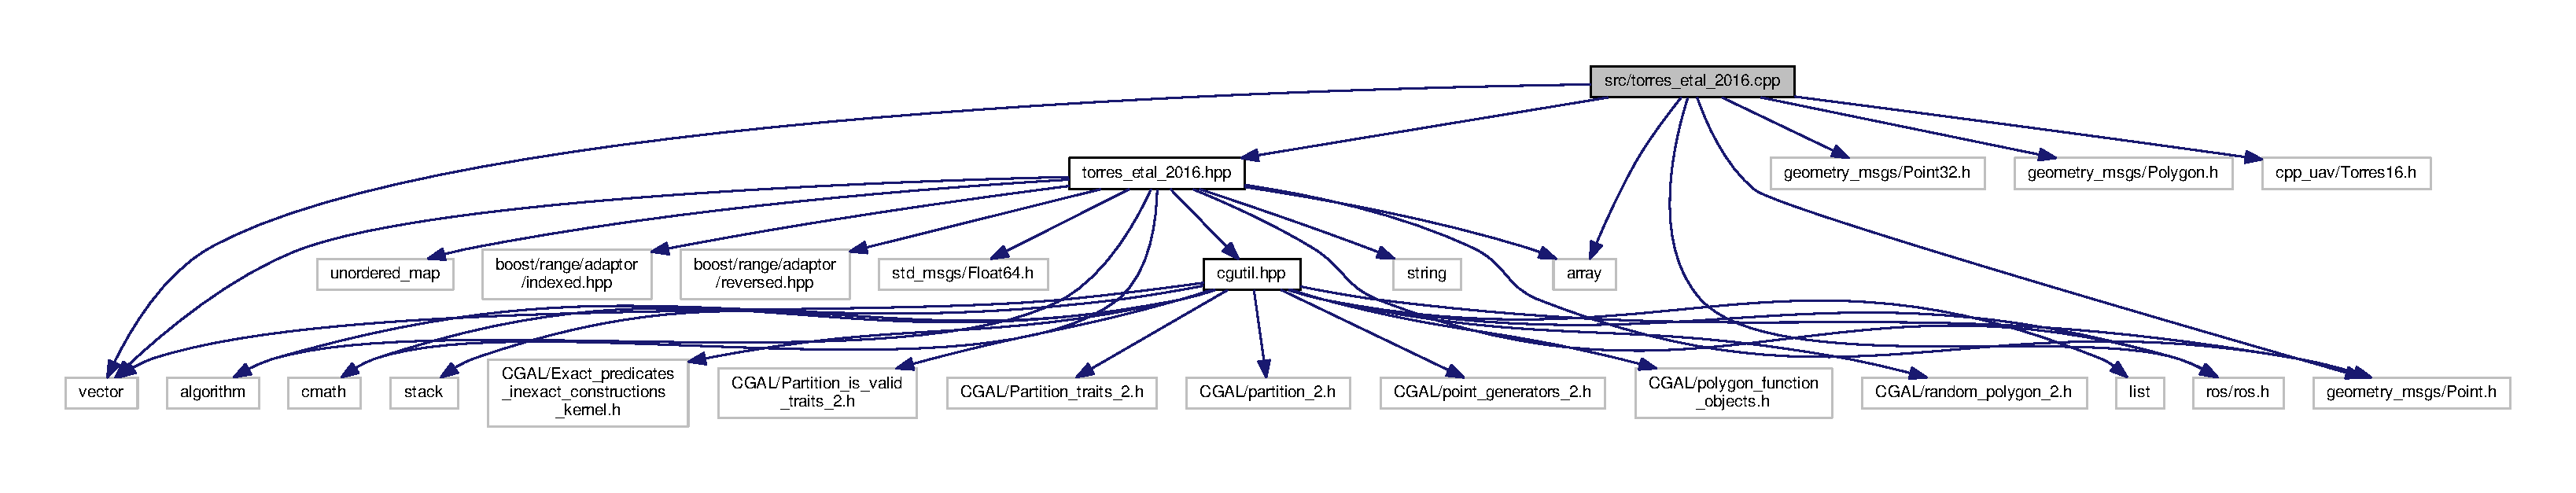
\includegraphics[width=350pt]{torres__etal__2016_8cpp__incl}
\end{center}
\end{figure}
\subsection*{Functions}
\begin{DoxyCompactItemize}
\item 
std\+::vector$<$ geometry\+\_\+msgs\+::\+Polygon $>$ \hyperlink{torres__etal__2016_8cpp_a423e5aed4b30f401e494d837996f3664}{generate\+Polygon\+Vector} (const \hyperlink{cgutil_8hpp_a23afdbfcb523553a73b329d7a91a7489}{Point\+Vector} \&polygon)
\begin{DoxyCompactList}\small\item\em Generate vector of polygon from Point\+Vector. \end{DoxyCompactList}\item 
std\+::vector$<$ geometry\+\_\+msgs\+::\+Polygon $>$ \hyperlink{torres__etal__2016_8cpp_abf23a92b5a7db75fa0c1f347207e4d3b}{generate\+Polygon\+Vector} (const std\+::vector$<$ \hyperlink{cgutil_8hpp_a23afdbfcb523553a73b329d7a91a7489}{Point\+Vector} $>$ \&sub\+Polygons)
\begin{DoxyCompactList}\small\item\em Generate vector of polygon from std\+::vector$<$\+Point\+Vector$>$ \end{DoxyCompactList}\item 
bool \hyperlink{torres__etal__2016_8cpp_a287cacfa0cf7ef5502045d26ec77bac0}{plan} (cpp\+\_\+uav\+::\+Torres16\+::\+Request \&req, cpp\+\_\+uav\+::\+Torres16\+::\+Response \&res)
\begin{DoxyCompactList}\small\item\em Plans coverage path. \end{DoxyCompactList}\item 
int \hyperlink{torres__etal__2016_8cpp_a3c04138a5bfe5d72780bb7e82a18e627}{main} (int argc, char $\ast$$\ast$argv)
\end{DoxyCompactItemize}


\subsection{Detailed Description}
Coverage path planner based on M. Torres et al, 2016. 

\begin{DoxyAuthor}{Author}
Takaki Ueno 
\end{DoxyAuthor}


\subsection{Function Documentation}
\index{torres\+\_\+etal\+\_\+2016.\+cpp@{torres\+\_\+etal\+\_\+2016.\+cpp}!generate\+Polygon\+Vector@{generate\+Polygon\+Vector}}
\index{generate\+Polygon\+Vector@{generate\+Polygon\+Vector}!torres\+\_\+etal\+\_\+2016.\+cpp@{torres\+\_\+etal\+\_\+2016.\+cpp}}
\subsubsection[{\texorpdfstring{generate\+Polygon\+Vector(const Point\+Vector \&polygon)}{generatePolygonVector(const PointVector &polygon)}}]{\setlength{\rightskip}{0pt plus 5cm}std\+::vector$<$geometry\+\_\+msgs\+::\+Polygon$>$ generate\+Polygon\+Vector (
\begin{DoxyParamCaption}
\item[{const {\bf Point\+Vector} \&}]{polygon}
\end{DoxyParamCaption}
)}\hypertarget{torres__etal__2016_8cpp_a423e5aed4b30f401e494d837996f3664}{}\label{torres__etal__2016_8cpp_a423e5aed4b30f401e494d837996f3664}


Generate vector of polygon from Point\+Vector. 


\begin{DoxyParams}{Parameters}
{\em polygon} & \\
\hline
\end{DoxyParams}
\begin{DoxyReturn}{Returns}
std\+::vector$<$geometry\+\_\+msgs\+::\+Polygon$>$ Vector of subpolygons assumed to be passed to R\+OS msg 
\end{DoxyReturn}
\index{torres\+\_\+etal\+\_\+2016.\+cpp@{torres\+\_\+etal\+\_\+2016.\+cpp}!generate\+Polygon\+Vector@{generate\+Polygon\+Vector}}
\index{generate\+Polygon\+Vector@{generate\+Polygon\+Vector}!torres\+\_\+etal\+\_\+2016.\+cpp@{torres\+\_\+etal\+\_\+2016.\+cpp}}
\subsubsection[{\texorpdfstring{generate\+Polygon\+Vector(const std\+::vector$<$ Point\+Vector $>$ \&sub\+Polygons)}{generatePolygonVector(const std::vector< PointVector > &subPolygons)}}]{\setlength{\rightskip}{0pt plus 5cm}std\+::vector$<$geometry\+\_\+msgs\+::\+Polygon$>$ generate\+Polygon\+Vector (
\begin{DoxyParamCaption}
\item[{const std\+::vector$<$ {\bf Point\+Vector} $>$ \&}]{sub\+Polygons}
\end{DoxyParamCaption}
)}\hypertarget{torres__etal__2016_8cpp_abf23a92b5a7db75fa0c1f347207e4d3b}{}\label{torres__etal__2016_8cpp_abf23a92b5a7db75fa0c1f347207e4d3b}


Generate vector of polygon from std\+::vector$<$\+Point\+Vector$>$ 


\begin{DoxyParams}{Parameters}
{\em polygon} & \\
\hline
\end{DoxyParams}
\begin{DoxyReturn}{Returns}
std\+::vector$<$geometry\+\_\+msgs\+::\+Polygon$>$ Vector of subpolygons assumed to be passed to R\+OS msg 
\end{DoxyReturn}
\index{torres\+\_\+etal\+\_\+2016.\+cpp@{torres\+\_\+etal\+\_\+2016.\+cpp}!main@{main}}
\index{main@{main}!torres\+\_\+etal\+\_\+2016.\+cpp@{torres\+\_\+etal\+\_\+2016.\+cpp}}
\subsubsection[{\texorpdfstring{main(int argc, char $\ast$$\ast$argv)}{main(int argc, char **argv)}}]{\setlength{\rightskip}{0pt plus 5cm}int main (
\begin{DoxyParamCaption}
\item[{int}]{argc, }
\item[{char $\ast$$\ast$}]{argv}
\end{DoxyParamCaption}
)}\hypertarget{torres__etal__2016_8cpp_a3c04138a5bfe5d72780bb7e82a18e627}{}\label{torres__etal__2016_8cpp_a3c04138a5bfe5d72780bb7e82a18e627}
\index{torres\+\_\+etal\+\_\+2016.\+cpp@{torres\+\_\+etal\+\_\+2016.\+cpp}!plan@{plan}}
\index{plan@{plan}!torres\+\_\+etal\+\_\+2016.\+cpp@{torres\+\_\+etal\+\_\+2016.\+cpp}}
\subsubsection[{\texorpdfstring{plan(cpp\+\_\+uav\+::\+Torres16\+::\+Request \&req, cpp\+\_\+uav\+::\+Torres16\+::\+Response \&res)}{plan(cpp_uav::Torres16::Request &req, cpp_uav::Torres16::Response &res)}}]{\setlength{\rightskip}{0pt plus 5cm}bool plan (
\begin{DoxyParamCaption}
\item[{cpp\+\_\+uav\+::\+Torres16\+::\+Request \&}]{req, }
\item[{cpp\+\_\+uav\+::\+Torres16\+::\+Response \&}]{res}
\end{DoxyParamCaption}
)}\hypertarget{torres__etal__2016_8cpp_a287cacfa0cf7ef5502045d26ec77bac0}{}\label{torres__etal__2016_8cpp_a287cacfa0cf7ef5502045d26ec77bac0}


Plans coverage path. 


\begin{DoxyParams}{Parameters}
{\em req\mbox{[}in\mbox{]}} & Contains values neccesary to plan a path \\
\hline
{\em res\mbox{[}out\mbox{]}} & Contains resulting path \\
\hline
\end{DoxyParams}
\begin{DoxyReturn}{Returns}
bool
\end{DoxyReturn}
For details of this service, cf. srv/\+Torres16.\+srv 
\hypertarget{test__cgutil_8cpp}{}\section{test/test\+\_\+cgutil.cpp File Reference}
\label{test__cgutil_8cpp}\index{test/test\+\_\+cgutil.\+cpp@{test/test\+\_\+cgutil.\+cpp}}


Test program for \hyperlink{cgutil_8hpp}{cgutil.\+hpp}.  


{\ttfamily \#include $<$cgutil.\+hpp$>$}\\*
{\ttfamily \#include $<$gtest/gtest.\+h$>$}\\*
{\ttfamily \#include $<$array$>$}\\*
{\ttfamily \#include $<$cmath$>$}\\*
{\ttfamily \#include $<$vector$>$}\\*
{\ttfamily \#include $<$geometry\+\_\+msgs/\+Point.\+h$>$}\\*
Include dependency graph for test\+\_\+cgutil.\+cpp\+:\nopagebreak
\begin{figure}[H]
\begin{center}
\leavevmode
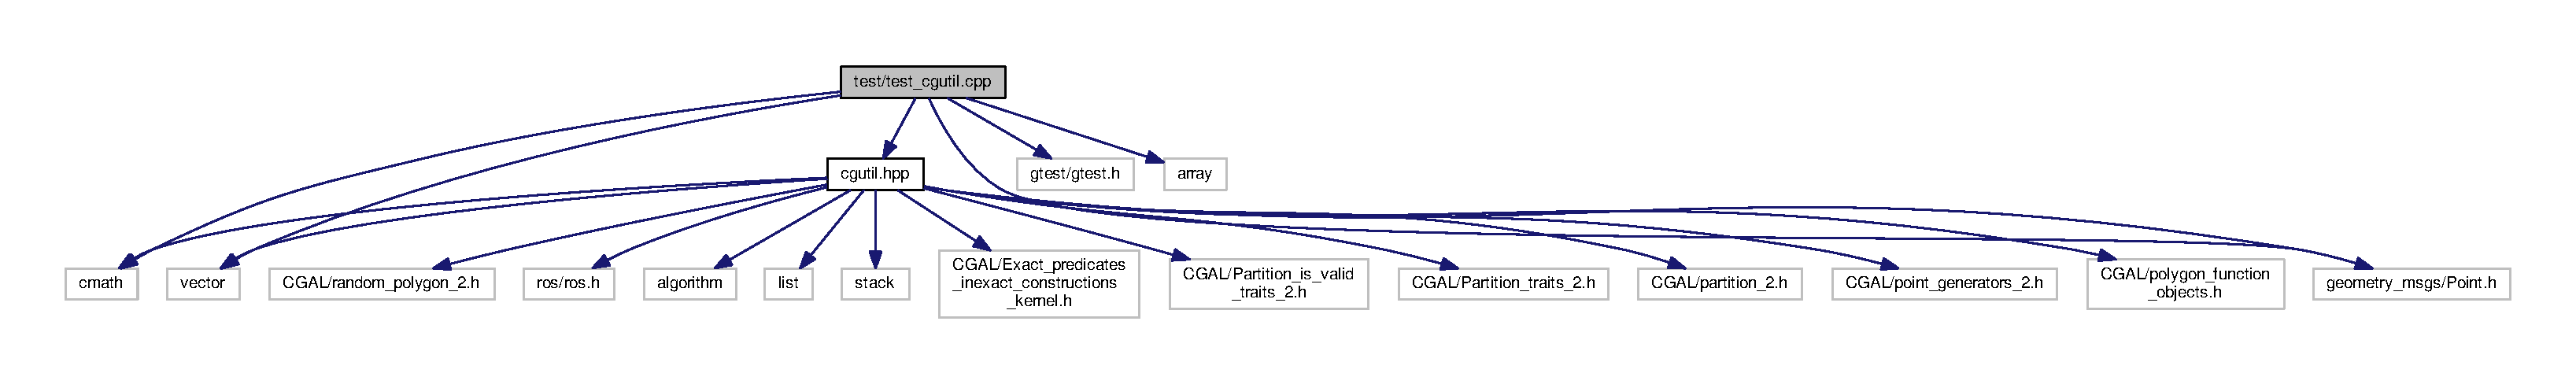
\includegraphics[width=350pt]{test__cgutil_8cpp__incl}
\end{center}
\end{figure}
\subsection*{Functions}
\begin{DoxyCompactItemize}
\item 
\hyperlink{test__cgutil_8cpp_a3d80ca900d90c35434f51286306329f0}{T\+E\+ST} (C\+G\+Util\+Test, Intersect\+Test1)
\item 
\hyperlink{test__cgutil_8cpp_a466bdeb395a53f1cfe4450e7b9014eaf}{T\+E\+ST} (C\+G\+Util\+Test, Intersect\+Test2)
\item 
\hyperlink{test__cgutil_8cpp_a9108fede978c27516f50d85b66edccdd}{T\+E\+ST} (C\+G\+Util\+Test, In\+Between\+Test)
\item 
\hyperlink{test__cgutil_8cpp_ae84f1cbf8c083cc8b850e1a54f3d506b}{T\+E\+ST} (C\+G\+Util\+Test, Calc\+Distance\+Test)
\begin{DoxyCompactList}\small\item\em Test for distance() \end{DoxyCompactList}\item 
\hyperlink{test__cgutil_8cpp_a5743d392382f065cbac9cad16f4e53d3}{T\+E\+ST} (C\+G\+Util\+Test, Calc\+Vertex\+Angle\+Test)
\begin{DoxyCompactList}\small\item\em Test for vertex\+Angle() \end{DoxyCompactList}\item 
\hyperlink{test__cgutil_8cpp_a41727e040608b62aecf2e9c24725d539}{T\+E\+ST} (C\+G\+Util\+Test, Calc\+Horizontal\+Angle\+Test)
\begin{DoxyCompactList}\small\item\em Test for horizontal\+Angle() \end{DoxyCompactList}\item 
\hyperlink{test__cgutil_8cpp_a5118c2ccdf0885b57f278b8e6d5d077d}{T\+E\+ST} (C\+G\+Util\+Test, Calcsigned\+Area\+Test)
\begin{DoxyCompactList}\small\item\em Test for signed\+Area() \end{DoxyCompactList}\item 
\hyperlink{test__cgutil_8cpp_ab5f334a769ed6522dc8523148e5b28af}{T\+E\+ST} (C\+G\+Util\+Test, Graham\+Scan\+Test)
\begin{DoxyCompactList}\small\item\em Test for graham\+Scan() \end{DoxyCompactList}\item 
\hyperlink{test__cgutil_8cpp_a409ac13056c7f1294c10fcfbd7df897f}{T\+E\+ST} (C\+G\+Util\+Test, Is\+Convex\+Test1)
\item 
\hyperlink{test__cgutil_8cpp_ae2669ba09313fbcf0912a9344f5cd7cc}{T\+E\+ST} (C\+G\+Util\+Test, Is\+Convex\+Test2)
\item 
int \hyperlink{test__cgutil_8cpp_a3c04138a5bfe5d72780bb7e82a18e627}{main} (int argc, char $\ast$$\ast$argv)
\end{DoxyCompactItemize}


\subsection{Detailed Description}
Test program for \hyperlink{cgutil_8hpp}{cgutil.\+hpp}. 

\begin{DoxyAuthor}{Author}
Takaki Ueno 
\end{DoxyAuthor}


\subsection{Function Documentation}
\index{test\+\_\+cgutil.\+cpp@{test\+\_\+cgutil.\+cpp}!main@{main}}
\index{main@{main}!test\+\_\+cgutil.\+cpp@{test\+\_\+cgutil.\+cpp}}
\subsubsection[{\texorpdfstring{main(int argc, char $\ast$$\ast$argv)}{main(int argc, char **argv)}}]{\setlength{\rightskip}{0pt plus 5cm}int main (
\begin{DoxyParamCaption}
\item[{int}]{argc, }
\item[{char $\ast$$\ast$}]{argv}
\end{DoxyParamCaption}
)}\hypertarget{test__cgutil_8cpp_a3c04138a5bfe5d72780bb7e82a18e627}{}\label{test__cgutil_8cpp_a3c04138a5bfe5d72780bb7e82a18e627}
\index{test\+\_\+cgutil.\+cpp@{test\+\_\+cgutil.\+cpp}!T\+E\+ST@{T\+E\+ST}}
\index{T\+E\+ST@{T\+E\+ST}!test\+\_\+cgutil.\+cpp@{test\+\_\+cgutil.\+cpp}}
\subsubsection[{\texorpdfstring{T\+E\+S\+T(\+C\+G\+Util\+Test, Intersect\+Test1)}{TEST(CGUtilTest, IntersectTest1)}}]{\setlength{\rightskip}{0pt plus 5cm}T\+E\+ST (
\begin{DoxyParamCaption}
\item[{C\+G\+Util\+Test}]{, }
\item[{Intersect\+Test1}]{}
\end{DoxyParamCaption}
)}\hypertarget{test__cgutil_8cpp_a3d80ca900d90c35434f51286306329f0}{}\label{test__cgutil_8cpp_a3d80ca900d90c35434f51286306329f0}
\index{test\+\_\+cgutil.\+cpp@{test\+\_\+cgutil.\+cpp}!T\+E\+ST@{T\+E\+ST}}
\index{T\+E\+ST@{T\+E\+ST}!test\+\_\+cgutil.\+cpp@{test\+\_\+cgutil.\+cpp}}
\subsubsection[{\texorpdfstring{T\+E\+S\+T(\+C\+G\+Util\+Test, Intersect\+Test2)}{TEST(CGUtilTest, IntersectTest2)}}]{\setlength{\rightskip}{0pt plus 5cm}T\+E\+ST (
\begin{DoxyParamCaption}
\item[{C\+G\+Util\+Test}]{, }
\item[{Intersect\+Test2}]{}
\end{DoxyParamCaption}
)}\hypertarget{test__cgutil_8cpp_a466bdeb395a53f1cfe4450e7b9014eaf}{}\label{test__cgutil_8cpp_a466bdeb395a53f1cfe4450e7b9014eaf}
\index{test\+\_\+cgutil.\+cpp@{test\+\_\+cgutil.\+cpp}!T\+E\+ST@{T\+E\+ST}}
\index{T\+E\+ST@{T\+E\+ST}!test\+\_\+cgutil.\+cpp@{test\+\_\+cgutil.\+cpp}}
\subsubsection[{\texorpdfstring{T\+E\+S\+T(\+C\+G\+Util\+Test, In\+Between\+Test)}{TEST(CGUtilTest, InBetweenTest)}}]{\setlength{\rightskip}{0pt plus 5cm}T\+E\+ST (
\begin{DoxyParamCaption}
\item[{C\+G\+Util\+Test}]{, }
\item[{In\+Between\+Test}]{}
\end{DoxyParamCaption}
)}\hypertarget{test__cgutil_8cpp_a9108fede978c27516f50d85b66edccdd}{}\label{test__cgutil_8cpp_a9108fede978c27516f50d85b66edccdd}
\index{test\+\_\+cgutil.\+cpp@{test\+\_\+cgutil.\+cpp}!T\+E\+ST@{T\+E\+ST}}
\index{T\+E\+ST@{T\+E\+ST}!test\+\_\+cgutil.\+cpp@{test\+\_\+cgutil.\+cpp}}
\subsubsection[{\texorpdfstring{T\+E\+S\+T(\+C\+G\+Util\+Test, Calc\+Distance\+Test)}{TEST(CGUtilTest, CalcDistanceTest)}}]{\setlength{\rightskip}{0pt plus 5cm}T\+E\+ST (
\begin{DoxyParamCaption}
\item[{C\+G\+Util\+Test}]{, }
\item[{Calc\+Distance\+Test}]{}
\end{DoxyParamCaption}
)}\hypertarget{test__cgutil_8cpp_ae84f1cbf8c083cc8b850e1a54f3d506b}{}\label{test__cgutil_8cpp_ae84f1cbf8c083cc8b850e1a54f3d506b}


Test for distance() 

\index{test\+\_\+cgutil.\+cpp@{test\+\_\+cgutil.\+cpp}!T\+E\+ST@{T\+E\+ST}}
\index{T\+E\+ST@{T\+E\+ST}!test\+\_\+cgutil.\+cpp@{test\+\_\+cgutil.\+cpp}}
\subsubsection[{\texorpdfstring{T\+E\+S\+T(\+C\+G\+Util\+Test, Calc\+Vertex\+Angle\+Test)}{TEST(CGUtilTest, CalcVertexAngleTest)}}]{\setlength{\rightskip}{0pt plus 5cm}T\+E\+ST (
\begin{DoxyParamCaption}
\item[{C\+G\+Util\+Test}]{, }
\item[{Calc\+Vertex\+Angle\+Test}]{}
\end{DoxyParamCaption}
)}\hypertarget{test__cgutil_8cpp_a5743d392382f065cbac9cad16f4e53d3}{}\label{test__cgutil_8cpp_a5743d392382f065cbac9cad16f4e53d3}


Test for vertex\+Angle() 

\index{test\+\_\+cgutil.\+cpp@{test\+\_\+cgutil.\+cpp}!T\+E\+ST@{T\+E\+ST}}
\index{T\+E\+ST@{T\+E\+ST}!test\+\_\+cgutil.\+cpp@{test\+\_\+cgutil.\+cpp}}
\subsubsection[{\texorpdfstring{T\+E\+S\+T(\+C\+G\+Util\+Test, Calc\+Horizontal\+Angle\+Test)}{TEST(CGUtilTest, CalcHorizontalAngleTest)}}]{\setlength{\rightskip}{0pt plus 5cm}T\+E\+ST (
\begin{DoxyParamCaption}
\item[{C\+G\+Util\+Test}]{, }
\item[{Calc\+Horizontal\+Angle\+Test}]{}
\end{DoxyParamCaption}
)}\hypertarget{test__cgutil_8cpp_a41727e040608b62aecf2e9c24725d539}{}\label{test__cgutil_8cpp_a41727e040608b62aecf2e9c24725d539}


Test for horizontal\+Angle() 

\index{test\+\_\+cgutil.\+cpp@{test\+\_\+cgutil.\+cpp}!T\+E\+ST@{T\+E\+ST}}
\index{T\+E\+ST@{T\+E\+ST}!test\+\_\+cgutil.\+cpp@{test\+\_\+cgutil.\+cpp}}
\subsubsection[{\texorpdfstring{T\+E\+S\+T(\+C\+G\+Util\+Test, Calcsigned\+Area\+Test)}{TEST(CGUtilTest, CalcsignedAreaTest)}}]{\setlength{\rightskip}{0pt plus 5cm}T\+E\+ST (
\begin{DoxyParamCaption}
\item[{C\+G\+Util\+Test}]{, }
\item[{Calcsigned\+Area\+Test}]{}
\end{DoxyParamCaption}
)}\hypertarget{test__cgutil_8cpp_a5118c2ccdf0885b57f278b8e6d5d077d}{}\label{test__cgutil_8cpp_a5118c2ccdf0885b57f278b8e6d5d077d}


Test for signed\+Area() 

\index{test\+\_\+cgutil.\+cpp@{test\+\_\+cgutil.\+cpp}!T\+E\+ST@{T\+E\+ST}}
\index{T\+E\+ST@{T\+E\+ST}!test\+\_\+cgutil.\+cpp@{test\+\_\+cgutil.\+cpp}}
\subsubsection[{\texorpdfstring{T\+E\+S\+T(\+C\+G\+Util\+Test, Graham\+Scan\+Test)}{TEST(CGUtilTest, GrahamScanTest)}}]{\setlength{\rightskip}{0pt plus 5cm}T\+E\+ST (
\begin{DoxyParamCaption}
\item[{C\+G\+Util\+Test}]{, }
\item[{Graham\+Scan\+Test}]{}
\end{DoxyParamCaption}
)}\hypertarget{test__cgutil_8cpp_ab5f334a769ed6522dc8523148e5b28af}{}\label{test__cgutil_8cpp_ab5f334a769ed6522dc8523148e5b28af}


Test for graham\+Scan() 

\index{test\+\_\+cgutil.\+cpp@{test\+\_\+cgutil.\+cpp}!T\+E\+ST@{T\+E\+ST}}
\index{T\+E\+ST@{T\+E\+ST}!test\+\_\+cgutil.\+cpp@{test\+\_\+cgutil.\+cpp}}
\subsubsection[{\texorpdfstring{T\+E\+S\+T(\+C\+G\+Util\+Test, Is\+Convex\+Test1)}{TEST(CGUtilTest, IsConvexTest1)}}]{\setlength{\rightskip}{0pt plus 5cm}T\+E\+ST (
\begin{DoxyParamCaption}
\item[{C\+G\+Util\+Test}]{, }
\item[{Is\+Convex\+Test1}]{}
\end{DoxyParamCaption}
)}\hypertarget{test__cgutil_8cpp_a409ac13056c7f1294c10fcfbd7df897f}{}\label{test__cgutil_8cpp_a409ac13056c7f1294c10fcfbd7df897f}
\index{test\+\_\+cgutil.\+cpp@{test\+\_\+cgutil.\+cpp}!T\+E\+ST@{T\+E\+ST}}
\index{T\+E\+ST@{T\+E\+ST}!test\+\_\+cgutil.\+cpp@{test\+\_\+cgutil.\+cpp}}
\subsubsection[{\texorpdfstring{T\+E\+S\+T(\+C\+G\+Util\+Test, Is\+Convex\+Test2)}{TEST(CGUtilTest, IsConvexTest2)}}]{\setlength{\rightskip}{0pt plus 5cm}T\+E\+ST (
\begin{DoxyParamCaption}
\item[{C\+G\+Util\+Test}]{, }
\item[{Is\+Convex\+Test2}]{}
\end{DoxyParamCaption}
)}\hypertarget{test__cgutil_8cpp_ae2669ba09313fbcf0912a9344f5cd7cc}{}\label{test__cgutil_8cpp_ae2669ba09313fbcf0912a9344f5cd7cc}

\hypertarget{test__torres__etal__2016_8cpp}{}\section{test/test\+\_\+torres\+\_\+etal\+\_\+2016.cpp File Reference}
\label{test__torres__etal__2016_8cpp}\index{test/test\+\_\+torres\+\_\+etal\+\_\+2016.\+cpp@{test/test\+\_\+torres\+\_\+etal\+\_\+2016.\+cpp}}


Test program for \hyperlink{torres__etal__2016_8hpp}{torres\+\_\+etal\+\_\+2016.\+hpp}.  


{\ttfamily \#include $<$torres\+\_\+etal\+\_\+2016.\+hpp$>$}\\*
{\ttfamily \#include $<$gtest/gtest.\+h$>$}\\*
{\ttfamily \#include $<$array$>$}\\*
{\ttfamily \#include $<$vector$>$}\\*
{\ttfamily \#include $<$geometry\+\_\+msgs/\+Point.\+h$>$}\\*
Include dependency graph for test\+\_\+torres\+\_\+etal\+\_\+2016.\+cpp\+:\nopagebreak
\begin{figure}[H]
\begin{center}
\leavevmode
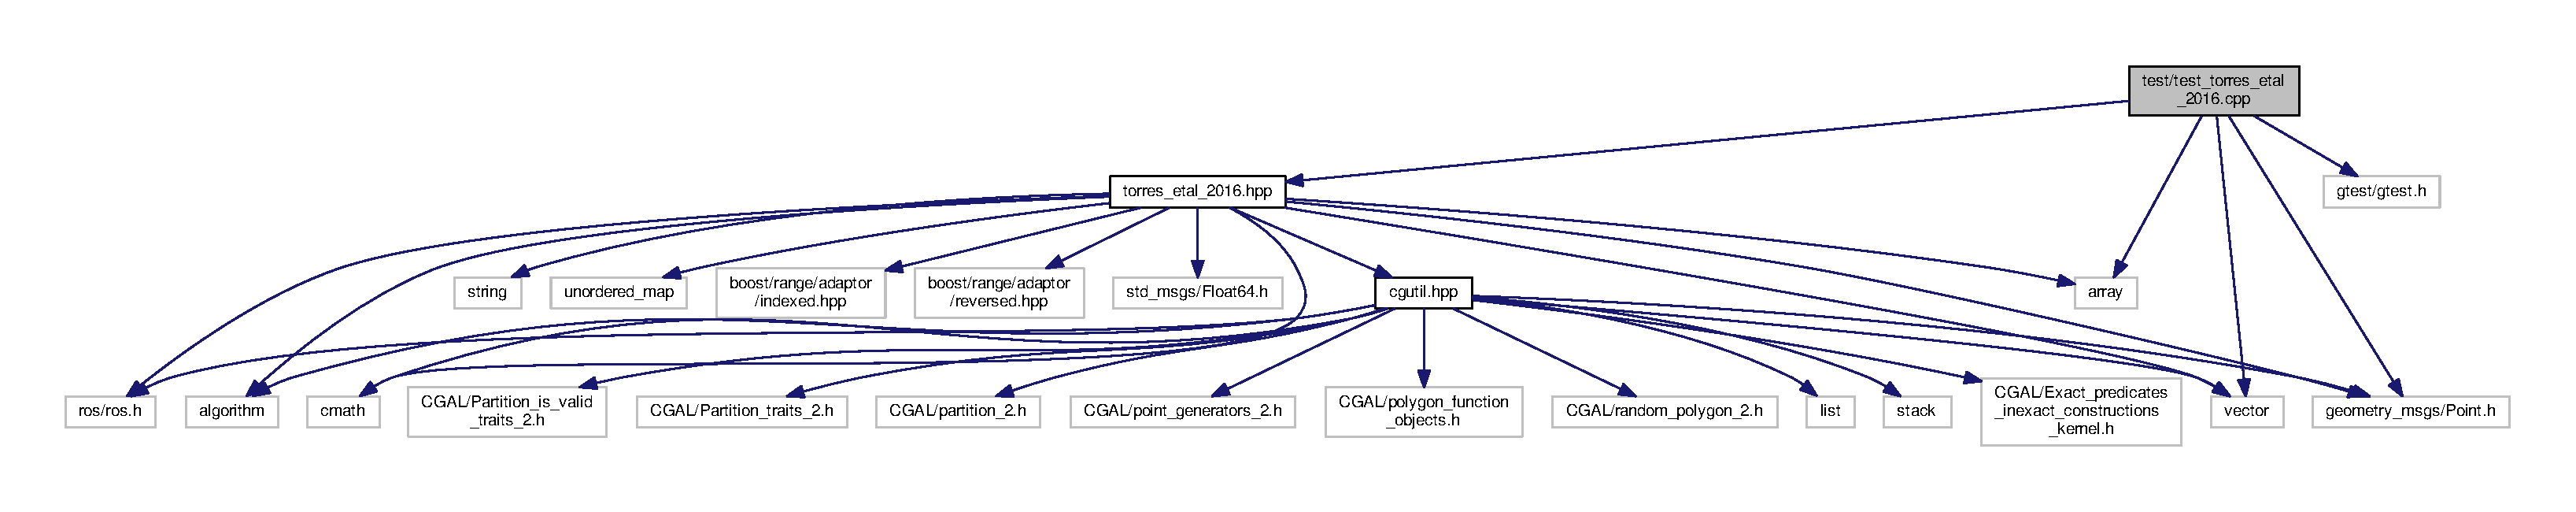
\includegraphics[width=350pt]{test__torres__etal__2016_8cpp__incl}
\end{center}
\end{figure}
\subsection*{Functions}
\begin{DoxyCompactItemize}
\item 
\hyperlink{test__torres__etal__2016_8cpp_a783e28ba207f6758ae2005320103c4e2}{T\+E\+ST} (Torres16\+Test, Calc\+Sweep\+Direction\+Test)
\begin{DoxyCompactList}\small\item\em Test for sweep\+Direction() \end{DoxyCompactList}\item 
int \hyperlink{test__torres__etal__2016_8cpp_a3c04138a5bfe5d72780bb7e82a18e627}{main} (int argc, char $\ast$$\ast$argv)
\end{DoxyCompactItemize}


\subsection{Detailed Description}
Test program for \hyperlink{torres__etal__2016_8hpp}{torres\+\_\+etal\+\_\+2016.\+hpp}. 

\begin{DoxyAuthor}{Author}
Takaki Ueno 
\end{DoxyAuthor}


\subsection{Function Documentation}
\index{test\+\_\+torres\+\_\+etal\+\_\+2016.\+cpp@{test\+\_\+torres\+\_\+etal\+\_\+2016.\+cpp}!main@{main}}
\index{main@{main}!test\+\_\+torres\+\_\+etal\+\_\+2016.\+cpp@{test\+\_\+torres\+\_\+etal\+\_\+2016.\+cpp}}
\subsubsection[{\texorpdfstring{main(int argc, char $\ast$$\ast$argv)}{main(int argc, char **argv)}}]{\setlength{\rightskip}{0pt plus 5cm}int main (
\begin{DoxyParamCaption}
\item[{int}]{argc, }
\item[{char $\ast$$\ast$}]{argv}
\end{DoxyParamCaption}
)}\hypertarget{test__torres__etal__2016_8cpp_a3c04138a5bfe5d72780bb7e82a18e627}{}\label{test__torres__etal__2016_8cpp_a3c04138a5bfe5d72780bb7e82a18e627}
\index{test\+\_\+torres\+\_\+etal\+\_\+2016.\+cpp@{test\+\_\+torres\+\_\+etal\+\_\+2016.\+cpp}!T\+E\+ST@{T\+E\+ST}}
\index{T\+E\+ST@{T\+E\+ST}!test\+\_\+torres\+\_\+etal\+\_\+2016.\+cpp@{test\+\_\+torres\+\_\+etal\+\_\+2016.\+cpp}}
\subsubsection[{\texorpdfstring{T\+E\+S\+T(\+Torres16\+Test, Calc\+Sweep\+Direction\+Test)}{TEST(Torres16Test, CalcSweepDirectionTest)}}]{\setlength{\rightskip}{0pt plus 5cm}T\+E\+ST (
\begin{DoxyParamCaption}
\item[{Torres16\+Test}]{, }
\item[{Calc\+Sweep\+Direction\+Test}]{}
\end{DoxyParamCaption}
)}\hypertarget{test__torres__etal__2016_8cpp_a783e28ba207f6758ae2005320103c4e2}{}\label{test__torres__etal__2016_8cpp_a783e28ba207f6758ae2005320103c4e2}


Test for sweep\+Direction() 


%--- End generated contents ---

% Index
\backmatter
\newpage
\phantomsection
\clearemptydoublepage
\addcontentsline{toc}{chapter}{Index}
\printindex

\end{document}
